\documentclass[12pt,a4paper]{article}
\usepackage[slovene]{babel}
\usepackage[utf8]{inputenc}
\usepackage{amsmath}
\usepackage{amsthm}
\usepackage{graphicx}
\usepackage{mdframed}
\usepackage{float}
\usepackage{url}
\usepackage{authblk}

\theoremstyle{definition}
\newenvironment{zgled}{%
  \begin{mdframed}[linewidth=0.5pt, topline=true, bottomline=true, leftline=true, rightline=true, 
                  innertopmargin=\baselineskip, innerbottommargin=\baselineskip]%
  \textbf{Zgled.}%
}{%
  \end{mdframed}%
}

\begin{document}

\setlength{\parskip}{1em}
\setlength{\parindent}{0pt}

\title{Analiza učinkovitosti javnega sektorja na primeru javnega zdravstva v Sloveniji in ZDA}
\author{Vid Boncelj Trošt, Vid Hočevar, Urh Videčnik, Tilen Žabkar}
\date{\today}
\affil{Fakulteta za matematiko in fiziko, Univerza v Ljubljani}
\maketitle

\begin{abstract}
    Namen naše naloge je oceniti učinkovitost ameriške in slovenske javne
    uprave. Tega smo se lotili s CRR modelom DEA analize. Zaradi oblike modela
    smo se osredotočili samo na zdravstvo. V teoretičnem
    delu smo spoznali osnovno idejo DEA analize in kako se uporablja za 
    izboljšanje učinkovitosti. Izpostavili smo tudi pomankljivosti DEA. 
    V praktičnem delu smo s pomočjo CRR indeksa in Malmquistovega indeksa
    ugotovili, da v zdravstvu v Sloveniji in ZDA produktivnost raste v zadnjih
    25 letih raste, najbolj produktiven čas pa je bil čas epidemije COVID-19. 
\end{abstract}

\newpage

\begingroup
\setlength{\parskip}{5pt}
\tableofcontents
\endgroup

\newpage

\section{Teoretični del}

\subsection{Uvod}

V javnem sektorju, za razliko od zasebnega, profitabilnost
ni tako zelo pomembna. Pogosto njeno vlogo zamenja učinkovitost. 
Učinkovitost je stopnja pri kateri je zagotavljanje storitev maksimizirana pri omejenih 
virih. Včasih je merjena tudi obratno -- kot stopnja, pri kateri je uporaba virov 
minimizirana pri pogoju zadostne zagotovitve storitev. 

Javni sektor je pogosto obravnavan kot neučinkovit zaradi odsotnosti
tekmovanja na trgu. Pričakovanja nam pravijo, da v primeru, ko obstajata
javna in zasebna storitev, bo javna manj učinkovita. To razmišljanje tudi
spodbuja gibanja v smer privatizacije javnih storitev v številnih državah.
Vendar je pomembno omeniti, da pogosto ne primerjamo primerljivih
storitev med javnim in zasebnim sektorjem. Namreč 
pogosto država zagotavlja blago in storitve ravno tam, kjer je trg odpovedal.
\cite{Lovell2002}

Vlade lahko zagotavljajo osnovne socialne storitve na področjih
zdravstva, izobraževanja in varnosti. Te storitve se financirajo
iz državenga proračuna (ki se financira iz davkov ter državenga
dolga) in ne prek zaračunavanja storitev. 

Številne študije so pokazale, da tako organizacije iz javnega
kot tudi zasebnega sektorja ne uporabljajo svojih omejenih virov
učinkovito. Možna posledica je, da bi prerazporeditev virov iz
zagotavljanja blaga in storitev, ki imajo razmeroma nizke
mejne družbene koristi, k tistim z razmeroma visokimi mejnimi
družbenimi koristmi, izboljšala splošno družbeno blaginjo.
Druga posledica je, da viri niso uporabljeni na najbolj 
produktiven način; to pomeni, da je mogoče proizvesti več
blaga in storitev brez dodatnih virov. \cite{Yaisawarng2002}

\subsection{Teoretično ogrodje}

Vladne agencije običajno vključujejo več enot za izvajanje 
storitev, ki zagotavljajo osnovne socialne storitve. 
Primer take delitve lahko vidimo na sliki 
\ref{fig:government_structure}.


\begin{figure}[htbp]
    \centering
    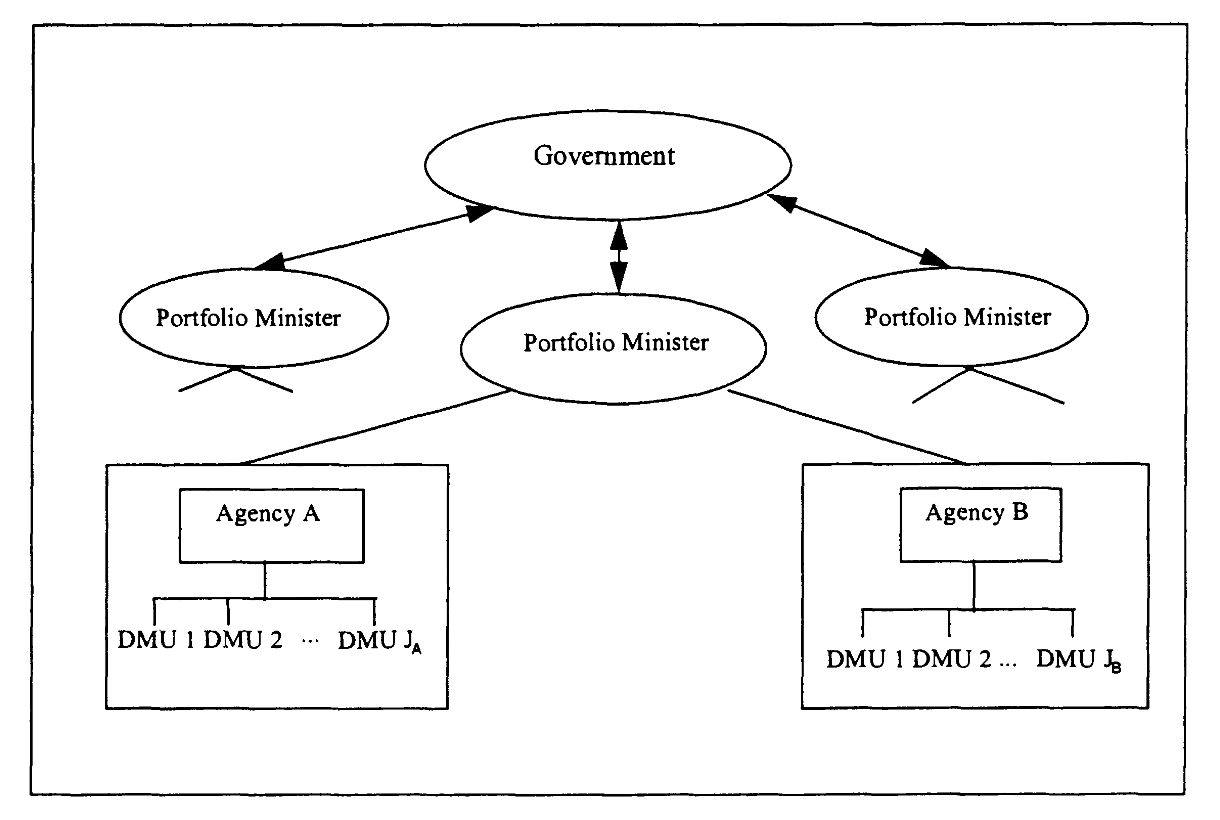
\includegraphics[width=0.7\textwidth]{government_structure.png}
    \caption{Struktura agencij v splošnem vladnem sektorju}
    \label{fig:government_structure}
    \vspace{0.2em}
    \footnotesize{Vir: \cite{Lovell2002}}
\end{figure}

Agenciji $A$ in $B$ sta odgovorni za zagotavljanje vladnih storitev, 
na primer ministrstvo za šolstvo (osnovno in srednješolsko 
izobraževanje) ter ministrstvo za delo (poklicno izobraževanje).
Agencija A vključuje $J_A$ osnovnih in srednjih šol, Agencija B 
pa $J_B$ izobraževalnih centrov. Delovanje teh agencij nadzoruje
pristojni minister. \cite{Yaisawarng2002}

\subsection{DEA analiza}

Analiza podatkovne ovojnice (\emph{angl.\ data envelopment analysis -- DEA}) je 
metoda linearnega programiranja, ki ustvari proizvodno mejo iz 
najproduktivnejših opazovanj v vzorcu. Ta meja predstavlja 
dejansko najboljšo prakso v naboru vključenih enot odločanja
(\emph{angl. decision making unit -- DMU}) in ne le teoretičnega optimuma. Ocena učinkovitosti 
vsake opazovane enote se izračuna glede na to mejo najboljše 
prakse. Ta postopek nam omogoča primerjavo uspešnosti različnih
enot, ki izvajajo podobne naloge, z najboljšimi izvajalci
v vzorcu. \cite{Yaisawarng2002}

Indeks učinkovitosti DEA je sestavljena mera uspešnosti,
ki upošteva vse vhodne in izhodne podatke v modelu ter služi
kot dopolnilno orodje k obstoječim meram produktivnosti,
kot npr.\ proizvod na delavca. Ocena učinkovitosti DEA
kaže delež trenutnih vhodov, ki
bi jih enota uporabila, če bi bila produktivno učinkovita,
ter nakazuje, ali se lahko določen vhod dodatno zmanjša brez
zmanjšanja drugih vhodov pri dani ravni izhodni vrednosti,
obenem pa zagotavlja nabor uteži, ki se uporabljajo za
oblikovanje ciljne točke za neučinkovito enoto. \cite{Yaisawarng2002}


\begin{figure}[htbp]
    \centering
    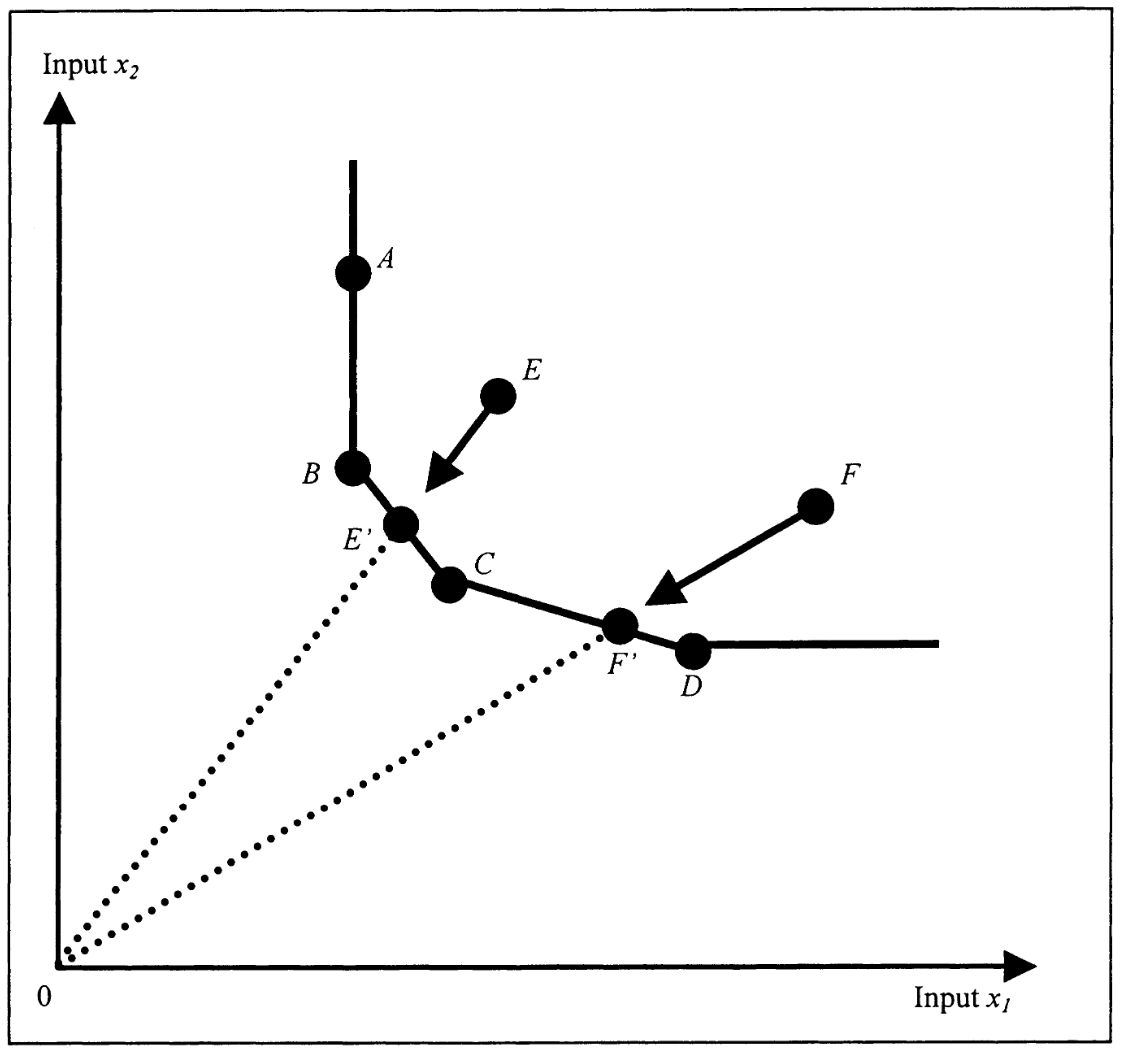
\includegraphics[width=0.7\textwidth]{dea_frontier.png}
    \caption{Proizvodna meja DEA}
    \label{fig:dea_frontier}
    \vspace{0.2em}
    \footnotesize{Vir: \cite{Lovell2002}}
\end{figure}

Slika \ref{fig:dea_frontier} predstavlja učinkovitost pri 
varčevanju z vložki za agencijo, sestavljeno iz šestih
DMU-jev, od $A$ do $F$. Vsak DMU proizvede enako količino
proizvoda $y$ pri uporabi različnih količin $x_1$ in $x_2$.
Za neučinkovit DMU $F$ velja $0F' < 0F$, oz.\ $0F'/0F < 1$,
kajti $F'$ je bližje izhodišču kot $F$. Če $F$ postane 
učinkovit, ob ohranitvi enakega razmerja vložkov, bo
na točki $F'$. Primera učinkovitih DMU-jev pa sta $C$
in $D$, ki imata višje razmerje med $y$ in $x_1$ ter
$x_2$, torej višje razmerje med vhodi in izhodi.

V tem primeru bi moral vodja neučinkovitega DMU-ja uporabiti
rezultate DEA kot vodilo pri razvoju načrta za izboljšanje
učinkovitosti. Postopek se začne z notranjo preiskavo DMU
za identifikacijo možnih razlag za prekomerno uporabo vhodnih sredstev.
Ta lahko identificira situacije, ki so specifične za ta DMU
in so zunaj nadzora vodje. V tem primeru se morajo te situacije
izvzeti iz DEA modela. Navedli bomo postopek, kako se DEA
lahko uporabi za izboljšanje učinkovitosti. \cite{Yaisawarng2002}
\newpage

\begin{enumerate}
    \item Uporabimo ocene učinkovitosti DEA in tako poiščemo
    vse neučinkovite DMU-je in obseg potencialnih izboljšav. 
    Identificiramo tudi učinkovite DMU-je, primerne za 
    primerjavo in specifična področja za preiskavo.
    
    \item Izvedemo preiskavo neučinkovitega 
    DMU-ja, da lahko določimo vzroke prekomerne 
    uporabe vhodnih sredstev.
    
    \item Posvetujemo se z primerljivimi učinkovitimi DMU-ji
    o njihovih koristnih praksah.
    
    \item Analiziramo kvalitativne in kvantitativne informacije
    iz preiskave in upoštevamo uteži primerjalnih enot DEA.
    
    \item Oblikujemo strateški načrt za implementacijo v 
    neučinkovitem DMU-ju. To lahko zahteva prestrukturiranje 
    organizacije in spremembe v upravljanju. \cite{Yaisawarng2002}
\end{enumerate}

\subsection{Uporaba DEA pri alokaciji sredstev}

Ocena učinkovitosti DEA se lahko uporablja pri razvoju
omejitev financiranja za vsak DMU. V primeru, ko cene
vložkov ne odražajo celotnih ekonomskih stroškov proizvodnje
(npr.\ zaradi državnih subvencij), lahko kot kazalnik 
uspešnosti raje uporabimo tehnično učinkovitost. 
\cite{Yaisawarng2002}

\begin{zgled}
    Oglejmo si triletni model odločanja. Odločamo se o količini sredstev, ki jih bo dobil DMU $A$. Predpostavimo, da so informacije o uspešnosti za 1.\ leto na voljo v 2.\ letu, preden se odločimo za proračun za 3.\ leto.

    Najprej predpostavimo, da je pričakovana raven
    zagotavljanja storitev za 3.\ leto enaka kot v 1.\
    letu. Prav tako predpostavimo, da poznamo ocene
    učinkovitosti za vse DMU-je v 1.\ letu. Za
    zagotavljanje storitev na učinkovit način lahko vsak
    DMU zaprosi za financiranje, ki je enako stroškom tehnično
    učinkovite ali najboljše prakse kombinacije vložkov.
    Denimo, da ima DMU $A$ proračun \$300{,}000 in oceno
    tehnične učinkovitosti enako 0{,}92. To pomeni, da bo v
    3.\ letu pričakovano, da $A$ uporabi kombinacijo vložkov
    najboljše prakse in zato dobi proračun $0{,}92 \times \$300{,}000 =
    \$276{,}000$.

    Dopustimo sedaj še spremembo povpraševanja po obstoječih
    storitvah. Dodatne storitve morajo biti zagotovljene
    z uporabo vložkov najboljše prakse. Predpostavimo,
    da se je povpraševanje po storitvah DMU $A$ povečalo
    za 10 odstotkov. Tedaj mora DMU $A$ prejeti dodatna
    sredstva v višini \$27{,}600 za prilagoditev 
    pričakovani rasti povpraševanja. Denimo, da je
    ocena dodatnih stroškov zaradi povečanega
    povpraševanja \$35{,}000. V tem primeru potrebuje
    DMU $A$ skupno $\$276{,}000 + \$27{,}600 + \$35{,}000
    = \$338{,}600$.
    
    Če seštejemo prošnje za financiranje po vseh DMU-jih
    znotraj agencije $r$, dobimo najmanjšo količino sredstev,
    ki jih potrebuje. \cite{Yaisawarng2002}
\end{zgled}

Vlada razporeja razpoložljive vire vsem agencijam 
javnega sektorja glede na svoje prioritete. Če so
skupna potrebna sredstva manjša od $\$X_B$, ki je na
voljo, lahko vlada ali ministri predlagajo nove 
programe ali naložbe. Nasprotno, če potrebna sredstva
presegajo $\$X_B$, kar je bolj običajno, vlada
zahteva, da ministri znotraj DMU-jev opravijo revizijo
in tako določijo pomembnejše naloge glede na prioritete
vlade ter potrebe skupnosti. Ta proces se ponavlja,
dokler se potrebna sredstva ne zmanjšajo pod $\$X_B$.

Alternativno lahko vlada uvede splošno zmanjšanje, ali
pa zahteva od agencij, da povečajo svojo učinkovitost.
Tako nekatere agencije prejmejo manj kot potrebujejo.
V takem primeru mora agencija $r$, ki je soočena z 
zmanjšanjem svojih sredstev, uporabiti splošno
zmanjšanje za vse DMU-je znotraj te agencije. To
pomeni omejitev nekaterih storitev in preklic
izvajanja novih. \mbox{Yaisawarng} predlaga, da
prilagoditve ravni storitev znotraj DMU-jev odobri
odgovorna agencija, skupne prilagoditve za agencijo
pa odobri vlada. Predlagani proces lahko ustvari 
pritisk na DMU, da poskušajo učinkovito uporabiti 
razpoložljive vire. 
\cite{Yaisawarng2002}

Oglejmo si različne načine za določanje ciljev DMU-jev.

\begin{table}[H]
    \centering
    \caption{Možne učinkovite kombinacije vhodov}
    \label{table:dmu_primer}
    \begin{tabular}{|l|c|c|c|}
    \hline
    & $A$ & $B$ & $C$ \\
    \hline
    Izhod/Vhod 1 & 14,3 & 16,7 & 12,5 \\
    Izhod/Vhod 2 & 5,7 & 5,0 & 6,7 \\
    Vhod 1/Vhod 2 & 0,4 & 0,3 & 0,53 \\
    \hline
    \end{tabular}
    \\ \vspace{0.2em}
    \footnotesize{Vir: \cite{Yaisawarng2002}}
\end{table}
    
\newpage

\begin{enumerate}
    \item[Možnost 1:] Ciljna ocena učinkovitosti za 
    DMU $A$ v 3.\ letu je najmanj 0{,}875, razmerja 
    izhod/vhod 1 in vhod 2 so najmanj 14,3 oziroma 5,7.
    
    \item[Možnost 2:] Ciljna ocena učinkovitosti za DMU
    $A$ v 3.\ letu je med 0{,}83 in 0{,}92, razmerje 
    izhod/vhod 1 je med 14,3 in 16,7, razmerje izhod/vhod 
    2 je med 5{,}7 in 6{,}7.
    
    \item[Možnost 3:] Ciljna ocena učinkovitosti za DMU
    $A$ v 3.\ letu je med 0{,}83 in 0{,}92, razmerje 
    izhod/vhod 1 je med 13{,}6 in 15, razmerje 
    izhod/vhod 2 je med 5{,}4 in 6{,}0.
\end{enumerate}

Tabela \ref{table:dmu_primer} predstavlja primer za ilustracijo
treh možnih alternativ za določanje primerjalnih
ciljev. Predpostavljamo, da DMU-ji uporabljajo dva
vhoda za proizvodnjo enega izhoda. Naj bo $A$ neučinkovit
DMU z radialno oceno učinkovitosti 0{,}875 v letu 1.
Poleg tega ima dva učinkovita vrstnika, imenovana 
$B$ in $C$. Možnost 1 določa ciljne delne mere za DMU
$A$ v 3.\ letu pri najboljši praksi kombinacije vložkov
$A$-ja glede na tehnologijo v letu 1. Te cilji 
predpostavljajo da $A$ lahko doseže stopnjo
izkoriščanja vložkov najboljše prakse pri konstantnem
razmerju tretnutnih vložkov. Ker je cilj učinkovitosti
postavljen na trenutni ravni vendar z višjim razmerjem
izhod-vhod, to pomeni, da se je proizvodna meja (Slika
\ref{fig:dea_frontier}) premaknila, kar pomeni tehnološki
napredek. \cite{Yaisawarng2002}

Možnosti 2 in 3 se od možnosti 1 razlikujeta v tem, da
določata primerjalne cilje kot interval in ne le kot točke.
Če predpostavimo, da agencija uporablja 5-odstotni pas 
dopustnih vrednosti, dobimo torej zaželeno vrednost 
učinkovitosti v letu 3 za $A$ med 0{,}83 in 0{,}92.
Možnost 2 se razlikuje še v tem, da uporablja
izhod-vhod razmerje na proizvodni meji DEA kot
spodnjo mejo ter večjega izmed razmerij učinkovitih
vrstnikov za zgornjo mejo. Možnost 3 uporabi 5-odstotni
pas okoli vrednosti na proizvodni meji DEA. 
\cite{Yaisawarng2002}

\subsection{Pomankljivosti DEA}

Seveda DEA model ne more vedno zajeti vseh pogledov
delovanje DMU-jev. Težava je lahko nedostopnost
podatkov ali pa napačna opredelitev modela.
Prav tako DEA ne dopušča šuma ali napak v podatkih.
Poleg tega se lahko zgodi, da so nekateri DMU-ji v
posameznem letu zelo učinkoviti zaradi sreče, ali pa
nasprotno, da zaradi težav zunaj njihovega nadzora
ne delujejo z največjim potencialom.

Model tudi predpostavlja, da lahko DMU-ji že skozi
proračunsko leto izboljšajo svojo učinkovitost. V
resnici potrebujejo ponavadi več obdobij za prilagoditev
in učenje. 

Preučimo lahko tudi predpostavko, da lahko z gotovostjo
napovemo rast povpraševanja na nekaterih področjih. Če
dejanska rast presega predvideno in bo DMU lahko vseeno
proizvajal na tej ravni brez dodatnih virov, ga bo
model označil za manj učinkovitega. Alternativno bi
lahko potrebovali dodatna sredstva.

Težavo lahko predstavlja tudi napredek v tehnologiji
skozi leto, ki ni bil napovedan v modelu. Kot posledico
lahko pomeni, da DMU-ji brez težav dosežejo svoje cilje,
ne da bi dejansko opravili potrebne spremembe. Zato se
mora rast tehnologije in produktivnosti predpostaviti 
in primerno spremeniti cilje.

Za konec omenimo še težavo v asimetriji informacij med
agencijami in vlado. Agencijam je namreč v interesu,
da zaprosijo za več sredstev, kolikor jih dejansko 
potrebujejo. 

\section{Praktični del}

Namen naše naloge je oceniti učinkovitost ameriške in slovenske
javne uprave. Ker je z DEA metodami smiselno
primerjati le DMU-je znotraj posameznih sektorjev, bomo v nalogi obravnavali le
javno zdravstvo. Za posamezen DMU bomo vzeli državo (torej ZDA in Slovenijo) v obdobju 
enega leta za obdobje 2000--2022.

Za obdelavo vhodnih in izhodnih podatkov bomo uporabili CRR 
(Charles-Cooper-Rhoads) metodo, ki se pogosto uporablja za 
ocenjevanje učinkovitosti v javnih sektorjih, kjer so DMU-ji podobnega obsega, saj 
predpostavlja, da se s podvajanjem vhodov učinkovitost podvoji. 
Metoda na podlagi vhodnih in izhodnih podatkov zgradi mejo učinkovitosti, kjer najuspešnejšemu DMU-ju pripiše vrednost 1,
najmanj uspešnemu pa vrednost 0. Druge DMU-je nato primerja z danima mejama in poda oceno od 0-1, ki jo
interpretiramo kot relativno učinkovitost na danem intervalu.

\subsection{Matematična formulacija CRR modela DEA}

Za vsako opazovano enoto \( o \) rešimo naslednji linearni program (vhodno orientiran model s konstantnim donosom na obseg):

\begin{align*}
\min_{\theta, \lambda} \quad & \theta \\
\text{p. p.} \quad 
& \sum_{j=1}^{n} \lambda_j x_{ij} \leq \theta x_{io}, \quad \forall i = 1, \dots, m \\
& \sum_{j=1}^{n} \lambda_j y_{rj} \geq y_{ro}, \quad \forall r = 1, \dots, s \\
& \lambda_j \geq 0, \quad \forall j = 1, \dots, n
\end{align*}

Kjer velja:
\begin{itemize}
    \item \( x_{ij} \) je vrednost vhodnega faktorja \( i \) za enoto \( j \),
    \item \( y_{rj} \) je vrednost izhodnega faktorja \( r \) za enoto \( j \),
    \item \( \lambda_j \) so uteži (kombinacija primerjalnih enot),
    \item \( \theta \) predstavlja oceno učinkovitosti (relativno tehnično učinkovitost enote \( o \)).
\end{itemize}

Če je \( \theta = 1 \), je enota učinkovita, sicer je neučinkovita in velja \( \theta < 1 \).

Poleg CRR metode bomo v nalogi uporabili še tako imenovani Malmquistovi indeks produktivnosti.
Pogosto se uporablja v analizi učinkovitosti med dvema časovnima obdobjema, poleg učinkovitosti
pa naj bi zaobjel tudi tehnološki napredek. Ker Malmquistov indeks
primerja le dve zaporedni obdobji (torej dva DMU-ja), ne spada pod DEA metode
(kjer so za konstrukcijo meje učinkovitosti potrebni najmanj 3 DMU-ji), se pa pogosto uporablja
v kobinaciji z DEA metodami. Za razliko od DEA metod pa ocenjuje relativno spremembo učinkovitosti 
(in tehnološkega napredka) glede na preteklo leto. 

CRR metoda vsakemu časovnemu obdobju pripiše indeks, ki je v primeru povečanja učinkovitosti glede
na prejšnje leto večji od 1, v primeru zmanjšanja učinkovitosti pa manjši od 1. Prvemu obdobju
indeksa ne pripišemo, saj služi za bazo, ki je ne moremo z ničimer primerjati. V našem primeru bo baza 
država v letu 2000, za vsa naslednja leta pa izračunamo indeks na podalgi prejšnjega.

\subsection{Malmquistov indeks produktivnosti}

Malmquistov indeks med obdobjema \( t \) in \( t+1 \) za določeno enoto se izračuna kot:

\begin{equation*}
M_0^{t,t+1} = \sqrt{
\left( \frac{D_t(x^{t+1}, y^{t+1})}{D_t(x^t, y^t)} \right)
\cdot
\left( \frac{D_{t+1}(x^{t+1}, y^{t+1})}{D_{t+1}(x^t, y^t)} \right)
}
\end{equation*}

Kjer je:
\begin{itemize}
    \item \( D_t(x^t, y^t) \) - funkcija razdalje glede na tehnologijo v obdobju \( t \),
    \item \( x^t, y^t \) - vhod in izhod v času \( t \),
    \item \( x^{t+1}, y^{t+1} \) - vhod in izhod v času \( t+1 \).
\end{itemize}

Indeks lahko zapišemo tudi kot produkt:
\[
M_0^{t,t+1} = \underbrace{\frac{D_{t+1}(x^{t+1}, y^{t+1})}{D_t(x^t, y^t)}}_{\text{Skupna sprememba učinkovitosti}}
= \underbrace{\frac{D_{t+1}(x^{t+1}, y^{t+1})}{D_t(x^{t+1}, y^{t+1})}}_{\text{Tehnološka sprememba}}
\times
\underbrace{\frac{D_t(x^{t+1}, y^{t+1})}{D_t(x^t, y^t)}}_{\text{Sprememba učinkovitosti}}
\]

\subsection{Analiza učinkovitosti javnega zdravstva v ZDA}

V skladu z metodologijo DEA smo za ocenjevanje učinkovitosti javnega sektorja v zdravstvu uporabili naslednje spremenljivke:

\begin{itemize}
\item Vhodne spremenljivke:
    \begin{itemize}
        \item Javna poraba kot delež BDP (v USD prilagojena glede na inflacijo, bazno leto 2010), ki odraža obseg javnih sredstev za zdravstvo.
        \item Število zdravnikov na 1000 prebivalcev, ki nam pokaže kadrovski vložek v zdravstveno oskrbo.
        \item Število zdravstvenega osebja na 1000 prebivalcev, ki kaže širši kadrovski obseg.
    \end{itemize}
\item Izhodne spremenljivke:
    \begin{itemize}
        \item Pričakovana življenjska doba posameznika, ki nam povzame dolgoročno učinkovitost določenega zdravstvenega sistema.
        \item Stopnja umrljivosti novorojenčkov, ki nam izraža kvaliteto in dostopnost do zdravstvene oskrbe.
    \end{itemize}
\end{itemize}

Izbira teh spremenljivk temelji na priporočilih v literaturi \cite{Yaisawarng2002} in nam omogoča realistično oceno učinkovitosti glede na težko pridobljene razpoložljive podatke.

\subsubsection{Poraba v zdravstvu}

Spodnji graf prikazuje gibanje javne in zasebne porabe za zdravstvo na prebivalca v ZDA v obdobju med letoma 2000 in 2022. 
Vrednosti so izražene v ameriških dolarjih in so prilagojene glede na inflacijo (bazno leto 2010), kar omogoča primerljivo analizo skozi čas.

\begin{figure}[H]
    \centering
    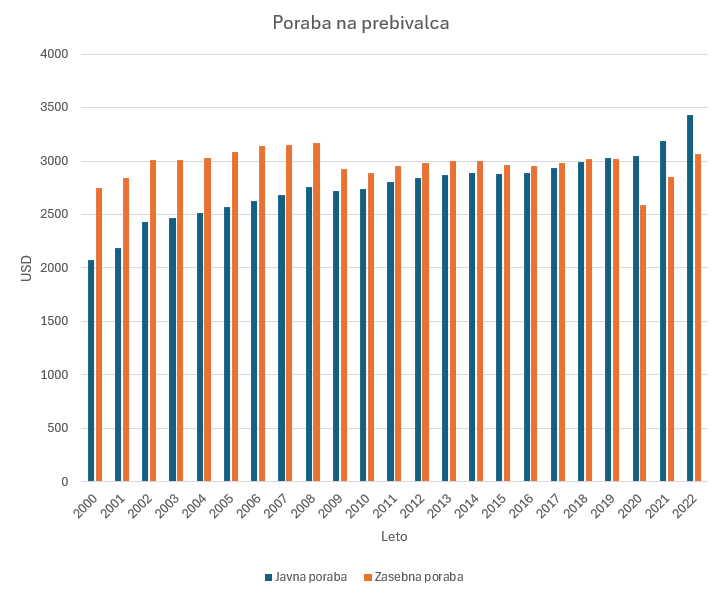
\includegraphics[width=0.7\textwidth]{zda_poraba_na_prebivalca.png}
    \caption{Poraba v zdravstvu na prebivalca v ZDA}
    \label{fig:zda_poraba_na_prebivalca}
\end{figure}

Opazimo lahko, da je bila zasebna poraba (npr.\ plačila iz žepa, zasebna zavarovanja) večino obdobja višja od javne, 
kar odraža strukturno naravnanost ameriškega zdravstvenega sistema k tržno financiranemu modelu. 
Do leta 2008 je bila zasebna poraba izrazito višja, nato pa se razlika začne zmanjševati. 
Posebno izstopata leto 2009, kjer pride do izrazitega padca zasebne porabe, zaradi gospodarske krize in leto 2020, 
kar je najverjetneje posledica pandemije COVID-19, ki je zmanjšala porabo zdravstvenih storitev pri zasebnem sektorju.

Po letu 2020 se trend obrne: javna poraba prehiti zasebno, 
kar lahko kaže na povečano vlogo države pri financiranju zdravstvenih ukrepov med pandemijo in po njej. 

Graf tako jasno pokaže, da struktura financiranja v ZDA ni stabilna, 
temveč se skozi čas prilagaja družbenim in ekonomskim razmeram.

Naseldnji graf prikazuje gibanje javne porabe za zdravstvo kot deleža BDP v ZDA med letoma 2000 in 2022. 
Opazimo lahko, da se je delež javne porabe postopoma povečeval. 
V začetku obdobja (okoli leta 2000) je znašal okrog $6 \%$ BDP, 
nato pa je v času gospodarske krize okoli leta 2009 močno narasel, 
kar je verjetno posledica večjih državnih izdatkov za zdravstvene in socialne programe.

\begin{figure}[H]
    \centering
    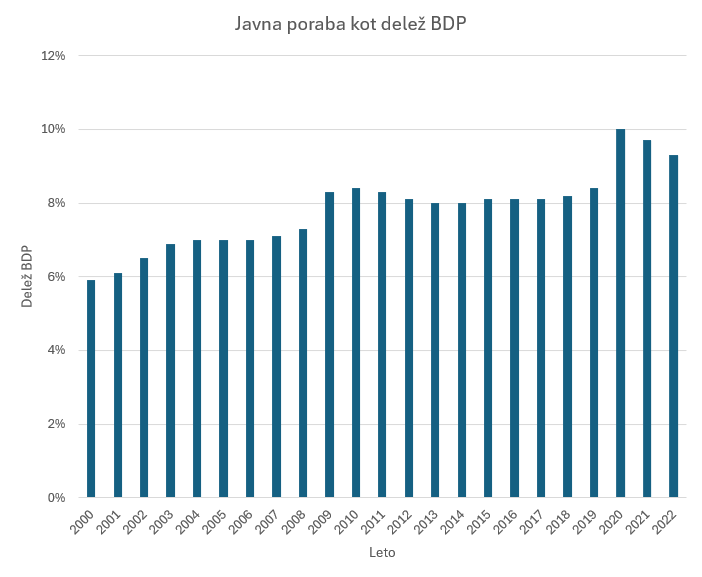
\includegraphics[width=0.7\textwidth]{zda_poraba_delez_BDP.png}
    \caption{Poraba v zdravstvu v ZDA kot delež BDP}
    \label{fig:zda_poraba_delez_BDP}
\end{figure}

V letih po krizi se delež stabilizira na ravni okoli $8\%$, nato pa v letu 2020 
ponovno izrazito poskoči, tokrat na približno $10\%$ BDP. Ta skok sovpada s pandemijo COVID-19, 
ko je vlada sprejela številne interventne ukrepe in povečala izdatke za zdravstveni sistem. 
V letih 2021 in 2022 se javna poraba nekoliko zniža, vendar ostaja višja kot pred pandemijo, 
kar nakazuje na trajnejši premik v vlogi države pri financiranju zdravstva.

Ta trend potrjuje ugotovitve iz prejšnje analize: v kriznih obdobjih (ekonomska recesija, pandemija) 
se država aktivneje vključuje v financiranje zdravstvenih storitev, kar vpliva na strukturo celotnega sistema. 
Povečan delež javne porabe pomeni večjo vlogo države in lahko vpliva tudi na učinkovitost in dostopnost zdravstvenega varstva.

\subsubsection{Število zdravnikov in zdravstvenega osebja}

Na spodnjem grafu želimo prikazati razvoj dveh ključnih kazalnikov kadrovskega vložka v zdravstveni sistem v ZDA: 
števila zdravnikov in števila zdravstvenega osebja na 1000 prebivalcev v obdobju 2000–2022.

\begin{figure}[H]
    \centering
    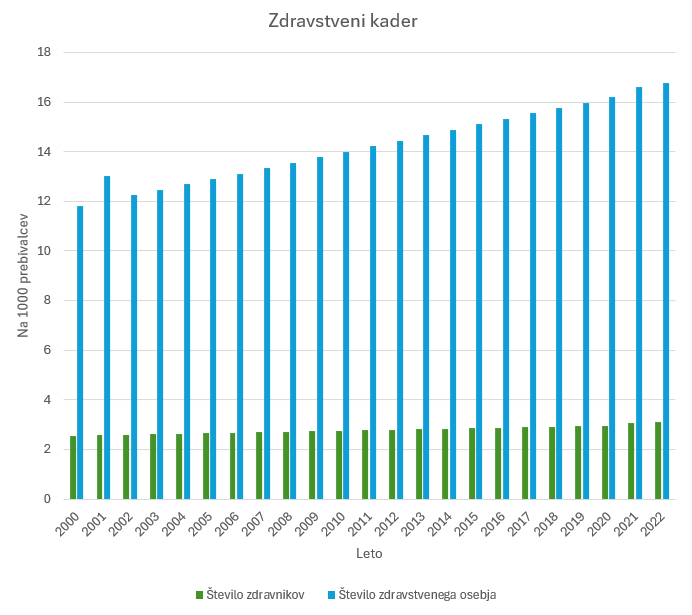
\includegraphics[width=0.7\textwidth]{zda_stevilo_zdravnikov.png}
    \caption{Število zdravnikov in zdravstvenega osebja na 1000 prebivalcev v ZDA}
    \label{fig:zda_stevilo_zdravnikov}
\end{figure}

Iz grafa je razvidno, da se je v zadnjih dveh desetletjih število obeh skupin sistematično povečevalo. 
Število zdravnikov se je postopno dvignilo z 2,56 na 3,12 zdravnika na 1000 prebivalcev (indeks 1,22). 
Še izrazitejši pa je trend pri širšem zdravstvenem osebju (ki vključuje medicinske sestre, tehnike, ...), 
kjer se je vrednost povečala iz približno 11,8 na 16,76 oseb na 1000 prebivalcev (indeks 1,42).

Ta rast je pomembna tudi za oceno učinkovitosti z metodo DEA, saj predstavljajo kadri enega izmed ključnih vhodov v analizi. 
Višji obseg kadrov pomeni večjo zmogljivost zdravstvenega sistema, vendar šele povezava z izhodnimi kazalniki 
(npr. življenjsko dobo) pokaže, ali je ta kadrovska širitev tudi učinkovita.

\subsubsection{Zdravstveni izidi}

Spodnja grafa prikazujeta dva ključna izhoda zdravstvenega sistema, to sta
pričakovana življenjska doba ter stopnja umrljivosti novorojenčkov (število smrti do 1. leta starosti na 1000 rojstev).

\begin{figure}[H]
    \centering
    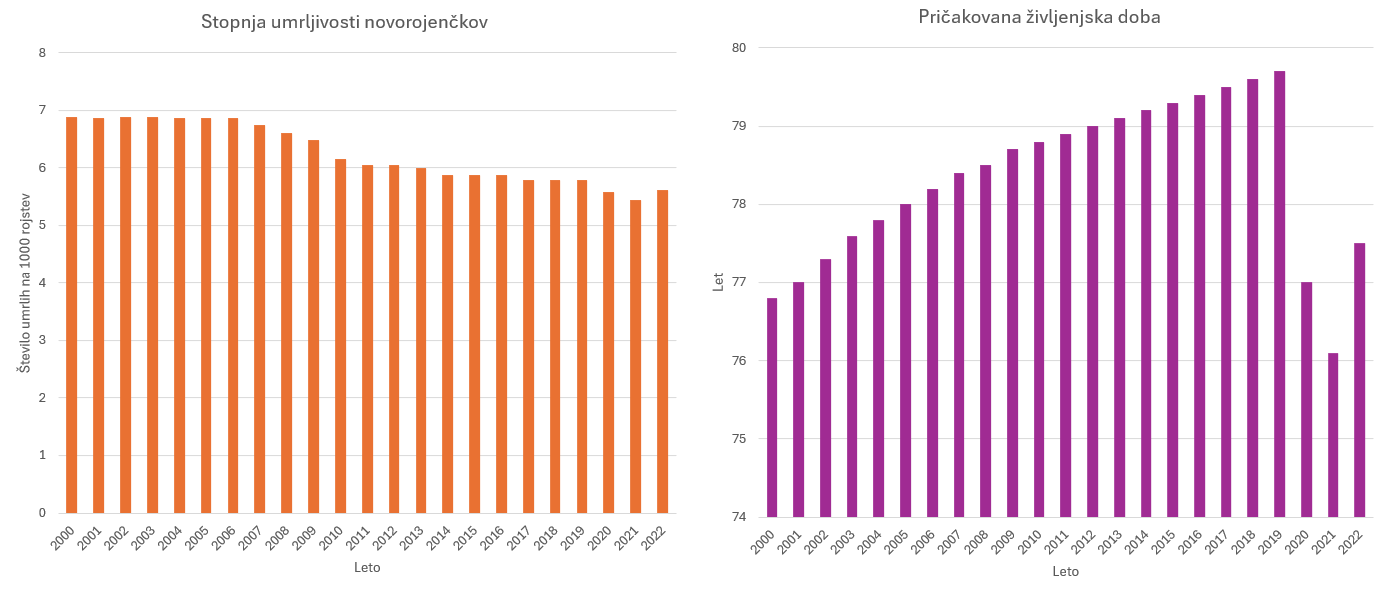
\includegraphics[width=0.9\textwidth]{zda_zdravstveni_izzidi.png}
    \caption{Zdravstveni izidi v ZDA}
    \label{fig:zda_zdravstveni_izzidi}
\end{figure}

Pričakovana življenjska doba v ZDA je od leta 2000 do 2019 naraščala, 
kar je kazalo na izboljšanje splošnega zdravstvenega stanja prebivalstva. 
V tem obdobju se je zvišala s 76,8 na skoraj 79,70 let. 
Vendar se je nato pojavil izrazit preobrat - med letoma 2020 in 2021 je pričakovana življenjska doba močno padla, 
kar sovpada s pandemijo COVID-19. Leta 2022 je zaznati rahlo okrevanje, vendar vrednost še ni dosegla predpandemijske ravni.

Stopnja umrljivosti novorojenčkov se je medtem ves čas postopno zmanjševala, iz približno 6,9 smrti do 1. leta starosti na 
1000 rojstev v letu 2000 na okoli 5,4 v letu 2020. 
Ta trend kaže na stalno izboljševanje v predporodni in poporodni zdravstveni oskrbi. 
V letu 2021 se pojavi majhno poslabšanje, 
kar lahko prav tako povezujemo s pandemijo in preobremenjenostjo zdravstvenega sistema, 
a je nivo v letu 2022 še vedno nižji kot pred dvema desetletjema.

\subsubsection{CRR indeks}
Model CRR primerja posamezna leta in na podlagi količine vložkov ter doseženih rezultatov ovrednoti relativno učinkovitost. 
Vrednost 1 pomeni najvišjo relativno učinkovitost, medtem ko vrednosti pod 1 pomenijo, 
kako učinkovito je bilo leto glede na najbolj učinkovito leto. Indeks 0,4213 za leto 2003 pomeni, 
da smo bili v tem letu le $42{,}13\%$ tako učinkoviti, kot v najbolj učinkovitem letu, ki ima indeks 1.

\begin{figure}[H]
    \centering
    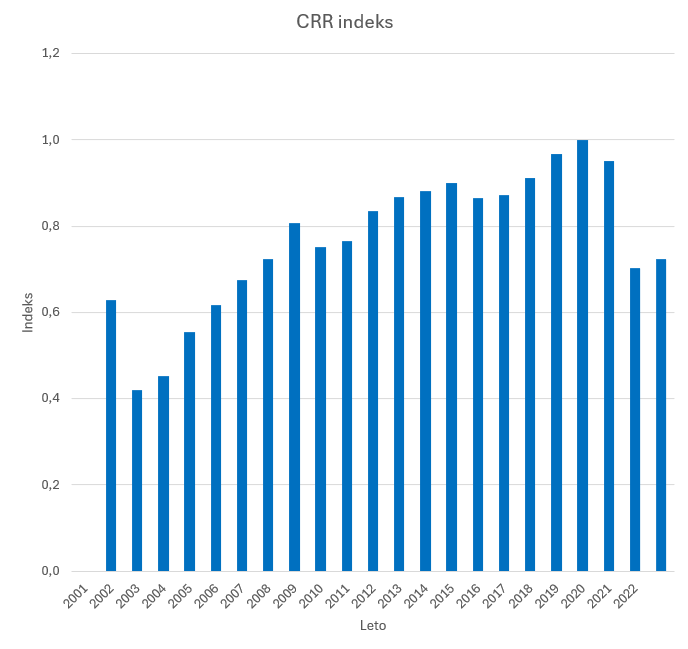
\includegraphics[width=0.7\textwidth]{zda_CRR_indeks.png}
    \caption{CRR indeks v ZDA}
    \label{fig:zda_CRR_indeks}
\end{figure}

Za vhodne podatke smo uporabili porabo javnega zdravstva kot delež bruto domačega proizvoda, 
število zdravnikov (na 1000 prebivalcev) in število zdravstvenega osebja (na 1000 prebivalcev). 
Pri izhodih pa smo preučili dva kazalnika, in sicer pričakovano življenjsko dobo in stopnjo umrljivosti dojenčkov, 
ki meri število umrlih otrok pred dopolnjenim prvim letom starosti na vaških 1000 rojenih otrok.

Iz grafa na sliki \ref{fig:zda_CRR_indeks} lahko razberemo, da z izjemo leta 2002 je produktivnost
naraščala in višek dosegla s COVID-19 epidemijo. Zanimiv je tudi padec produktivnosti po
ponovnem odprtju (2021 in 2022), kar bi lahko pripisali izčrpanosti
sistema in vrnitvi k običajnem stanju, kjer se ponovno izvajajo
manj učinkoviti posegi, ki so bili prekinjeni med epidemijo.

\subsubsection{Malmquistov indeks}

Malmquist indeks meri spremembo skupne produktivnosti med dvema zaporednima letoma. Vrednosti
nad 1 pomenijo napredek (več izhodov pri enakih ali manjših vhodih). Vrednosti enake 1 pomenijo stabilno produktivnost,
vrednosti pod 1 pa pomenijo upad produktivnosti. Indeks tako upošteva tako tehnološki napredek (npr.\ boljši postopki, digitalizacija),
kot tudi učinkovitostno prilagoditev (boljša organizacija ali raba virov).

\begin{figure}[H]
    \centering
    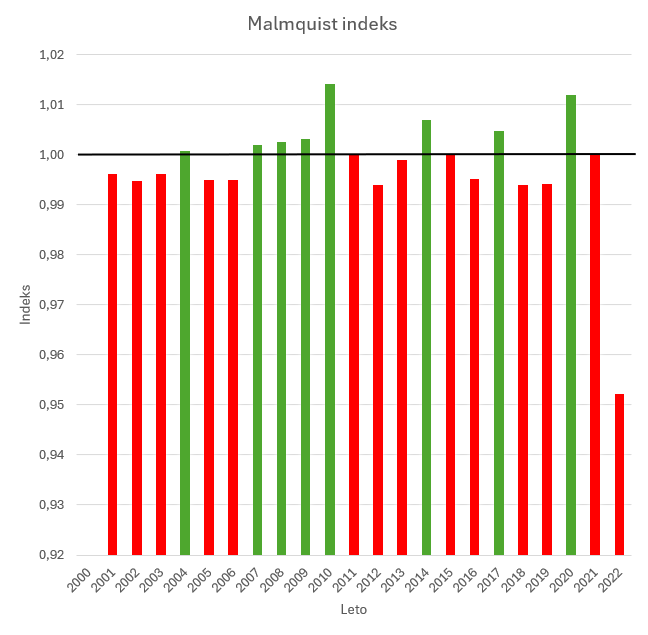
\includegraphics[width=0.7\textwidth]{zda_malmquist_indeks.png}
    \caption{Malmquist indeks v ZDA}
    \label{fig:zda_malmquist_indeks}
\end{figure}

V grafu je črna referenčna črta pri vrednosti 1, ki nam predstavlja mejo stabilnosti. 
Vidimo, da ZDA večino časa delujejo tik nad ali pod to vrednostjo, kar pomeni, 
da se spremembe produktivnosti dogajajo počasi in postopoma. 
Izjemen padec v letu 2022 pomeni, da je zdravstveni sistem (kljub morebitni rasti vhodov) 
ustvaril občutno manj učinkovite izide kot leto prej. Vzroke bi lahko
poiskali podobno, kot pri padcu produktivnosti v tem času, videnim s CRR
indeksom.

\subsection{Analiza učinkovitosti javnega zdravstva v Sloveniji}
\subsubsection{Poraba v zdravstvu}

Javna poraba namenjena zdravstvu je od preloma tisočletja nihala od dobre miljarde dolarjev letno, do več kot dveh miljard okoli leta 2010 in leta 2021. 
Če si števila ogledamo na prebivalca je vzorec enak, leta 2008, 2009, 2011 in 2021 izdatki sežejo nad dve miljardi dolarjev.
\begin{figure}[H]   % 'h' pomeni "here" - da se slika vstavi približno tukaj
    \centering       % centriranje slike
    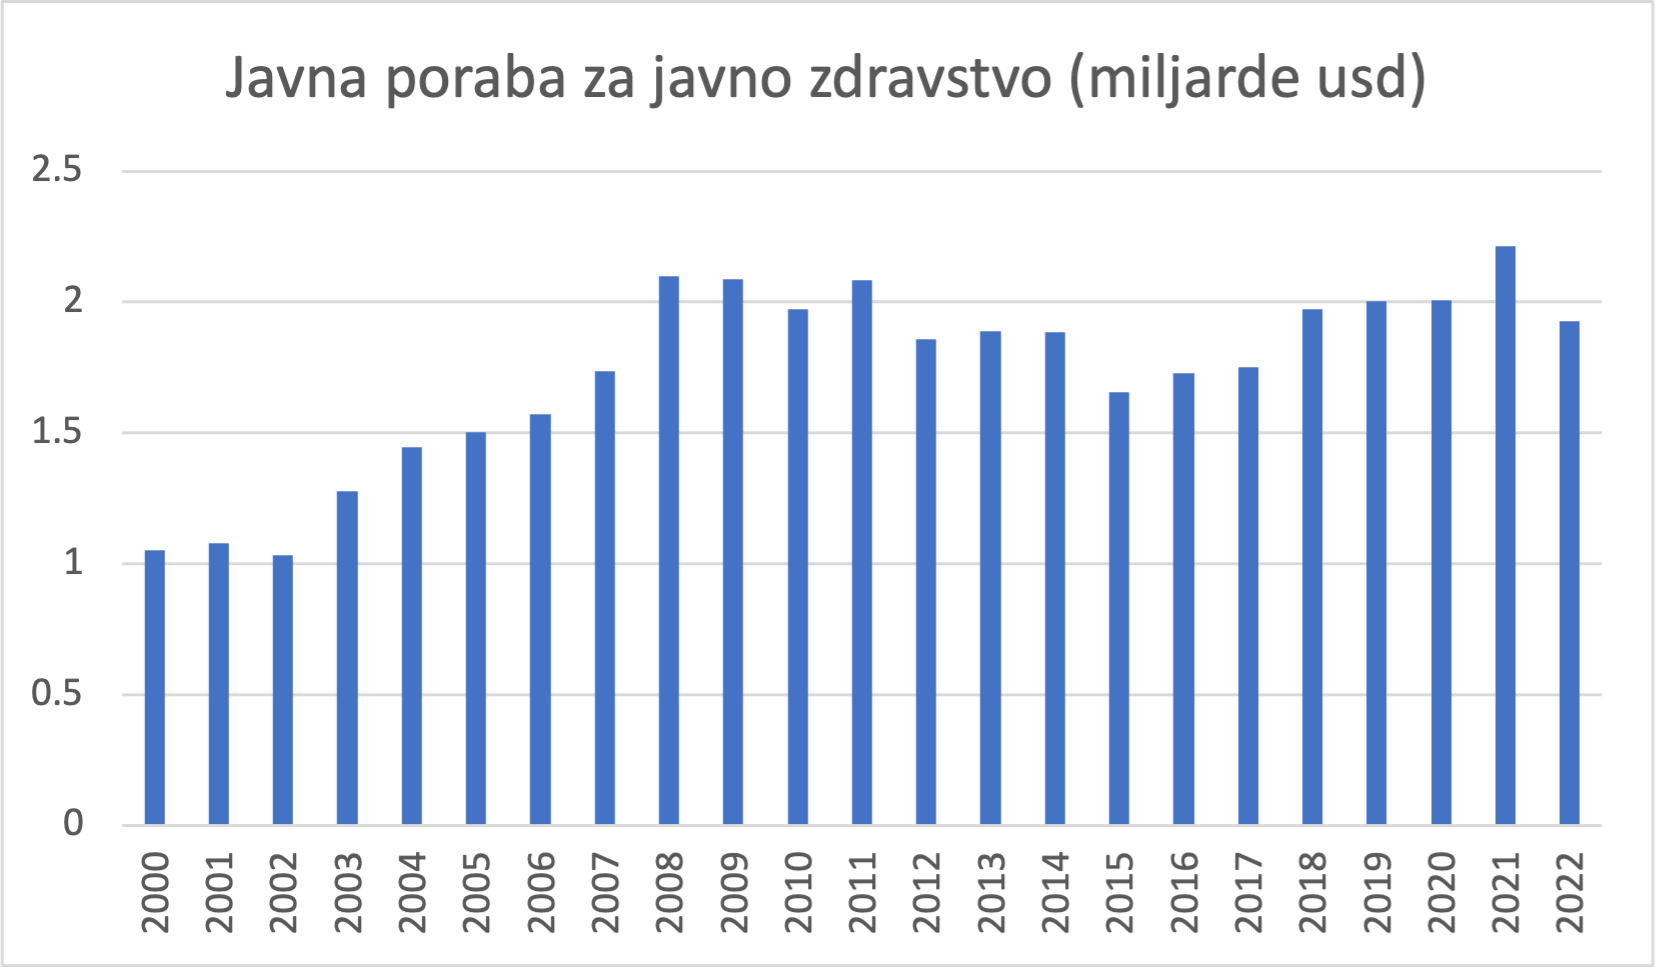
\includegraphics[width=0.7\textwidth]{jav_por_zdr_slo.png} % prilagodi širino po potrebi
    \caption{Javna poraba za javno zdravstvo v Sloveniji (v milijardah USD), prilagojena za inflacijo (bazno leto 2010), skozi čas}   % podnaslov slike (ni obvezno)
    \label{fig:jav_por_zdr_slo} % labela za sklicevanje na sliko (ni obvezno)
  \end{figure}

\begin{figure}[H]
    \centering
    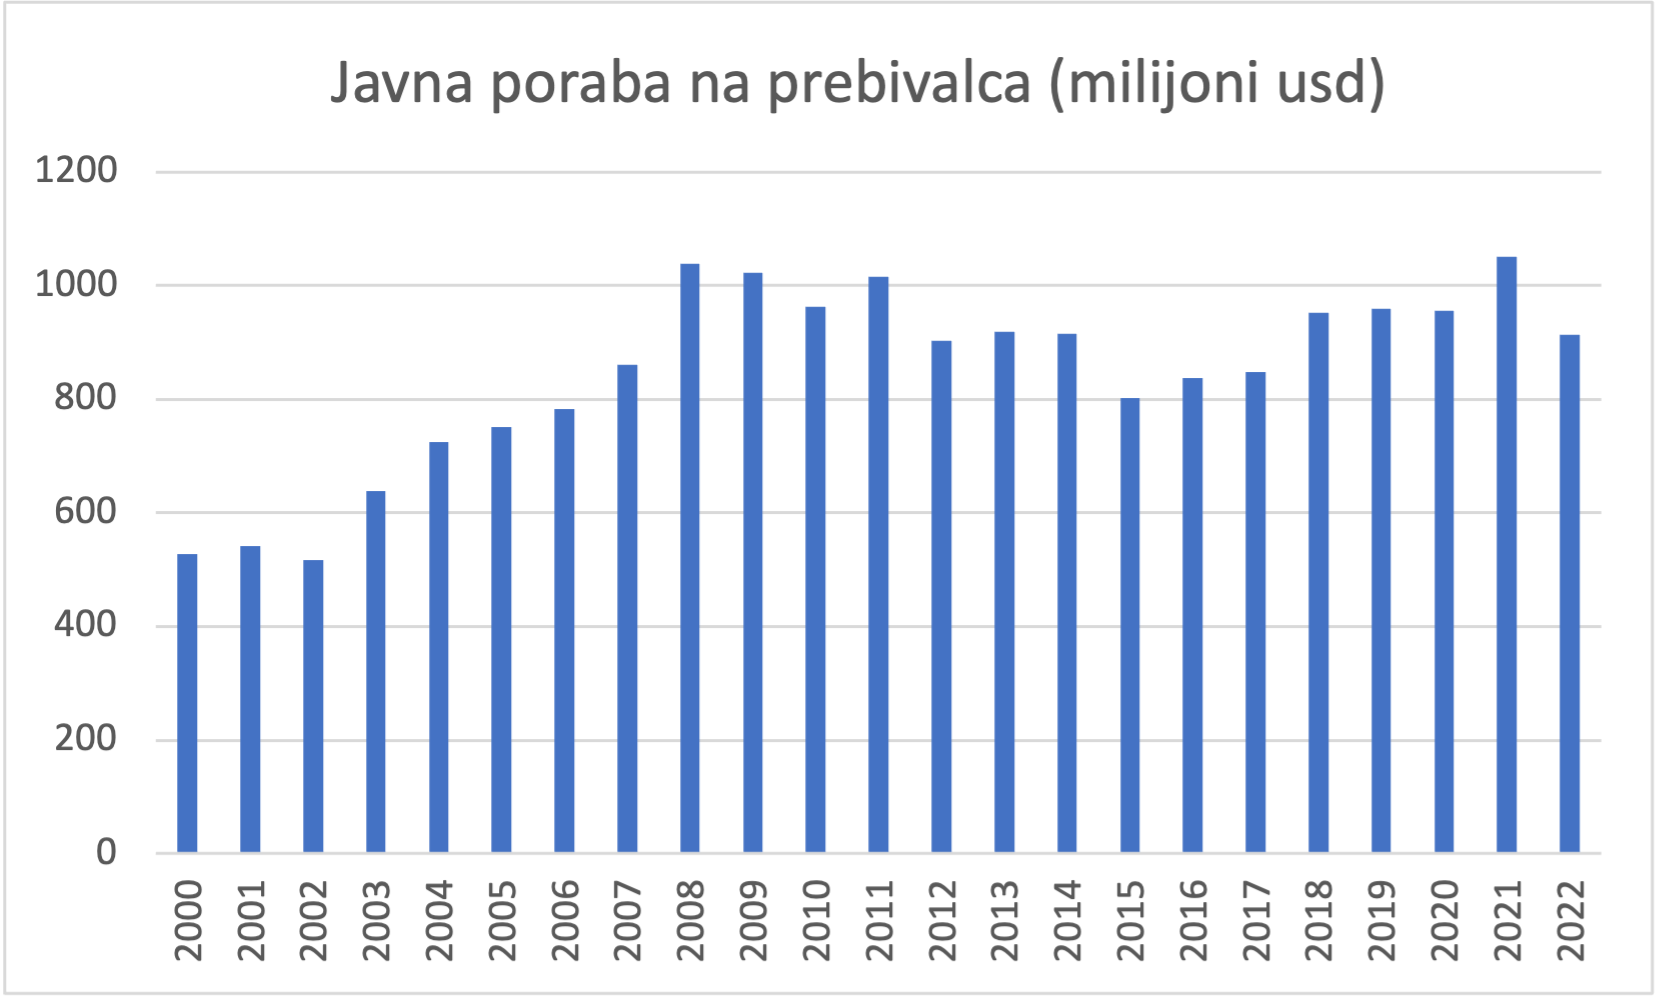
\includegraphics[width=0.7\textwidth]{jav_por_prb_slo.png}
    \caption{Javna poraba za javno zdravstvo v Sloveniji na prebivalca (v milijonih USD), prilagojena za inflacijo (bazno leto 2010), skozi čas}
    \label{fig:jav_por_prb_slo.png}
  \end{figure}

Slika je drugačna, če porabo ovrednotimo v okviru bruto domačega proizvoda. 
Vidimo, da javno financiranje zdravstva v zadnjih 20 letih konstantno narašča. 
Med letoma 2000 in 2022 se je tako povzpelo z 5,4 odstotka na kar 9,6 odstotka. 
Najbolj izrazit skok je bil med letoma 2019 in 2020 (za približno eno odstotno točko), kar je gotovo tudi posledica epidemije COVID-19. 
Kljub temu je naraščajoč trend viden že prej; do leta 2019 se je poraba namreč povečala za 3,1 odstotne točke.

\begin{figure}[H]
    \centering
    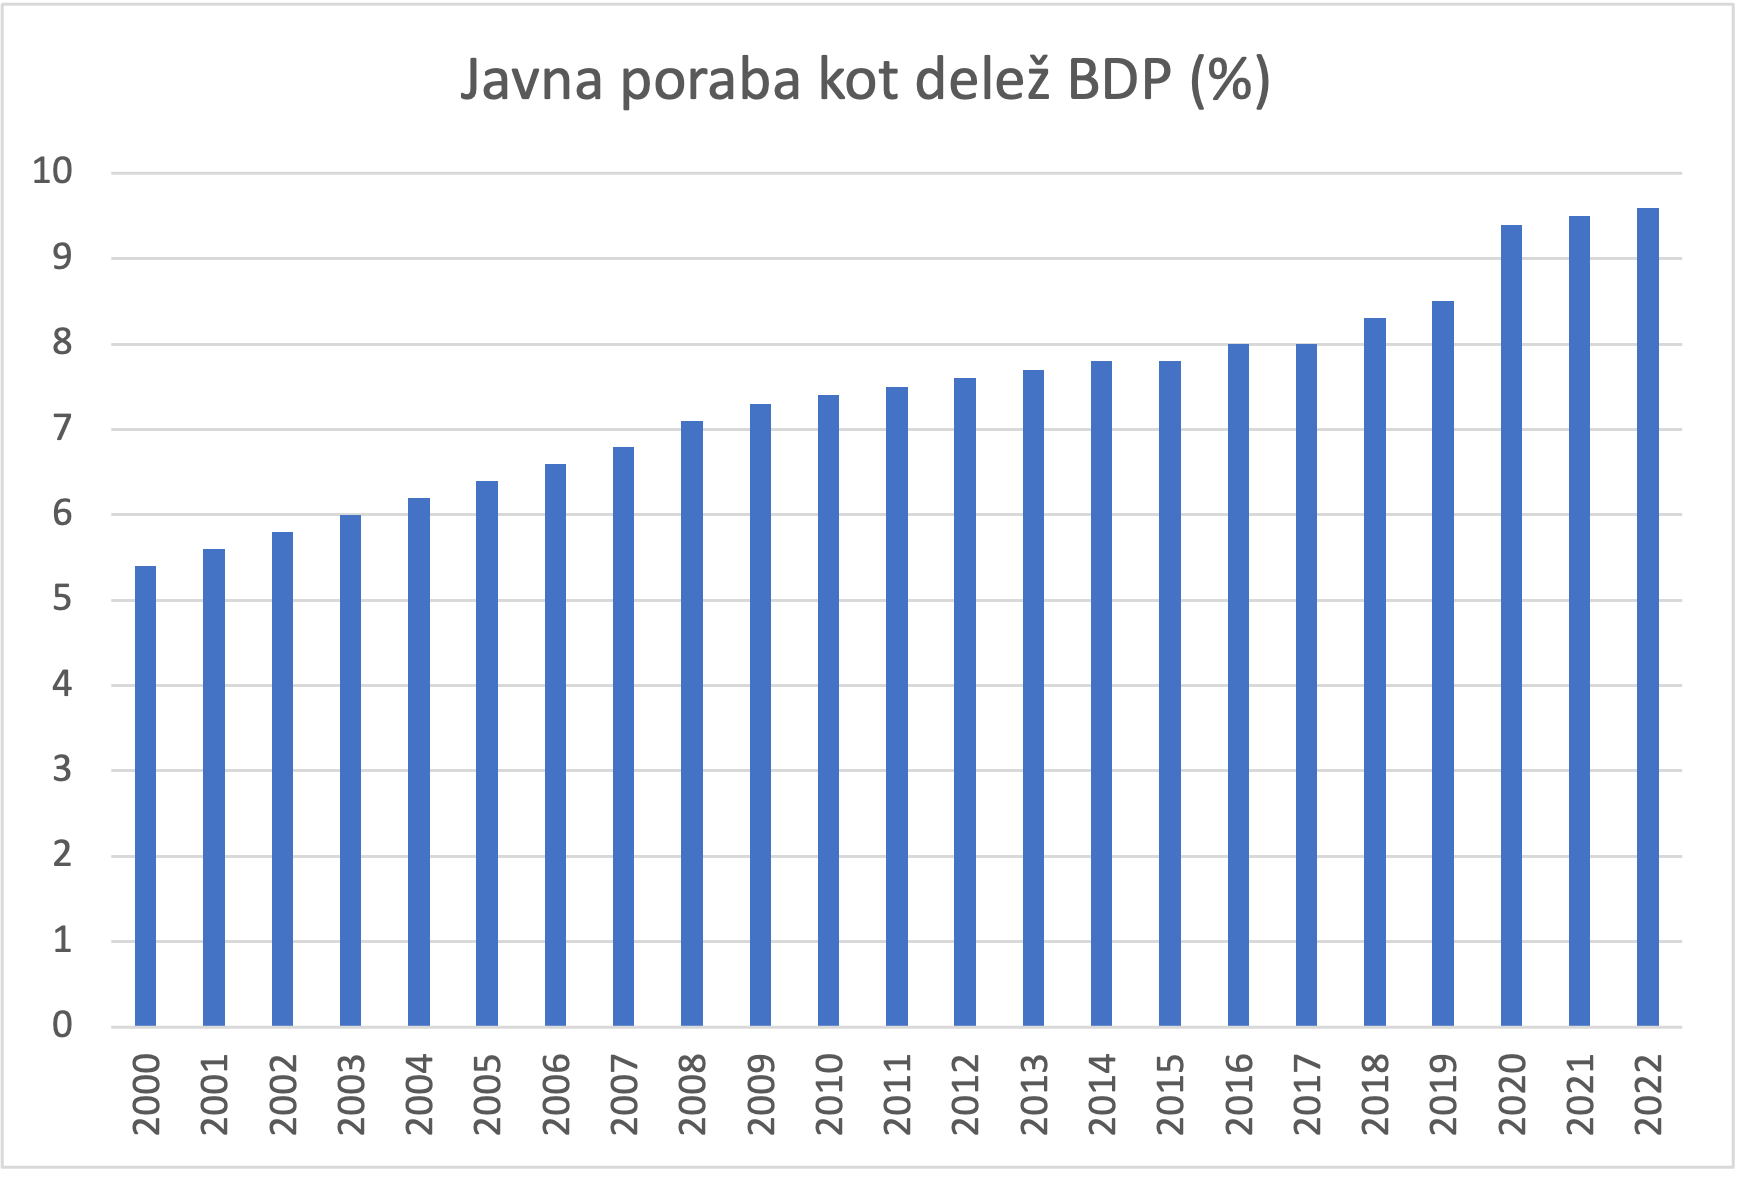
\includegraphics[width=0.7\textwidth]{jav_por_bdp_slo.png}
    \caption{Javna poraba za javno zdravstvo v Sloveniji kot delež bruto domačega proizvoda (v odstotkih), skozi čas}
    \label{fig:jav_por_bdp_slo.png}
  \end{figure}

Za povečanje izdatkov obstaja več razlogov. Prvi so demografske spremembe, natančneje staranje prebivalstva. 
Zelo hitro se povečujeta starostna odvisnost starejših od 65 let in vzdrževanost starejših od 85 let. 
Ob začetku tretjega desetletja enaindvajsetega stoletja imamo 35 prebivalcev, starih nad 65 let, na 100 delovno sposobnih, ter približno 13 prebivalcev, starih nad 85 let, na 100 prebivalcev, starih med 50 in 64 let.
Ob prelomu tisočletja sta bili obe številki nižji; starostna odvisnost je znašala dobrih 20, vzdrževanost starejših od 85 let pa manj kot deset. \cite{Sarec2023}
Opisane spremembe seveda povečujejo potrebe po zdravstvenih storitvah in dolgotrajni oskrbi.
  
Pomemben dejavnik rasti izdatkov je tudi razvoj tehnologije. 
Po ocenah Urada Republike Slovenije za makroekonomske analize in razvoj naj bi po različnih ocenah od 25 odstotkov do 75 odstotkov rasti izdatkov pojasnjevali s tehnološkim napredkom. \cite{zdravniska_zbornica_2023}

\subsubsection{Število zdravnikov in zdravstvenega osebja}

Za vhodne podatke smo uporabili porabo javnega zdravstva kot delež bruto domačega proizvoda, 
število zdravnikov (na 1000 prebivalcev) in število zdravstvenega osebja (na 1000 prebivalcev).
% Kaj spada pod zdravstveno osebje in od kod smo dobili podatke (vir)

\begin{figure}[H]
    \centering
    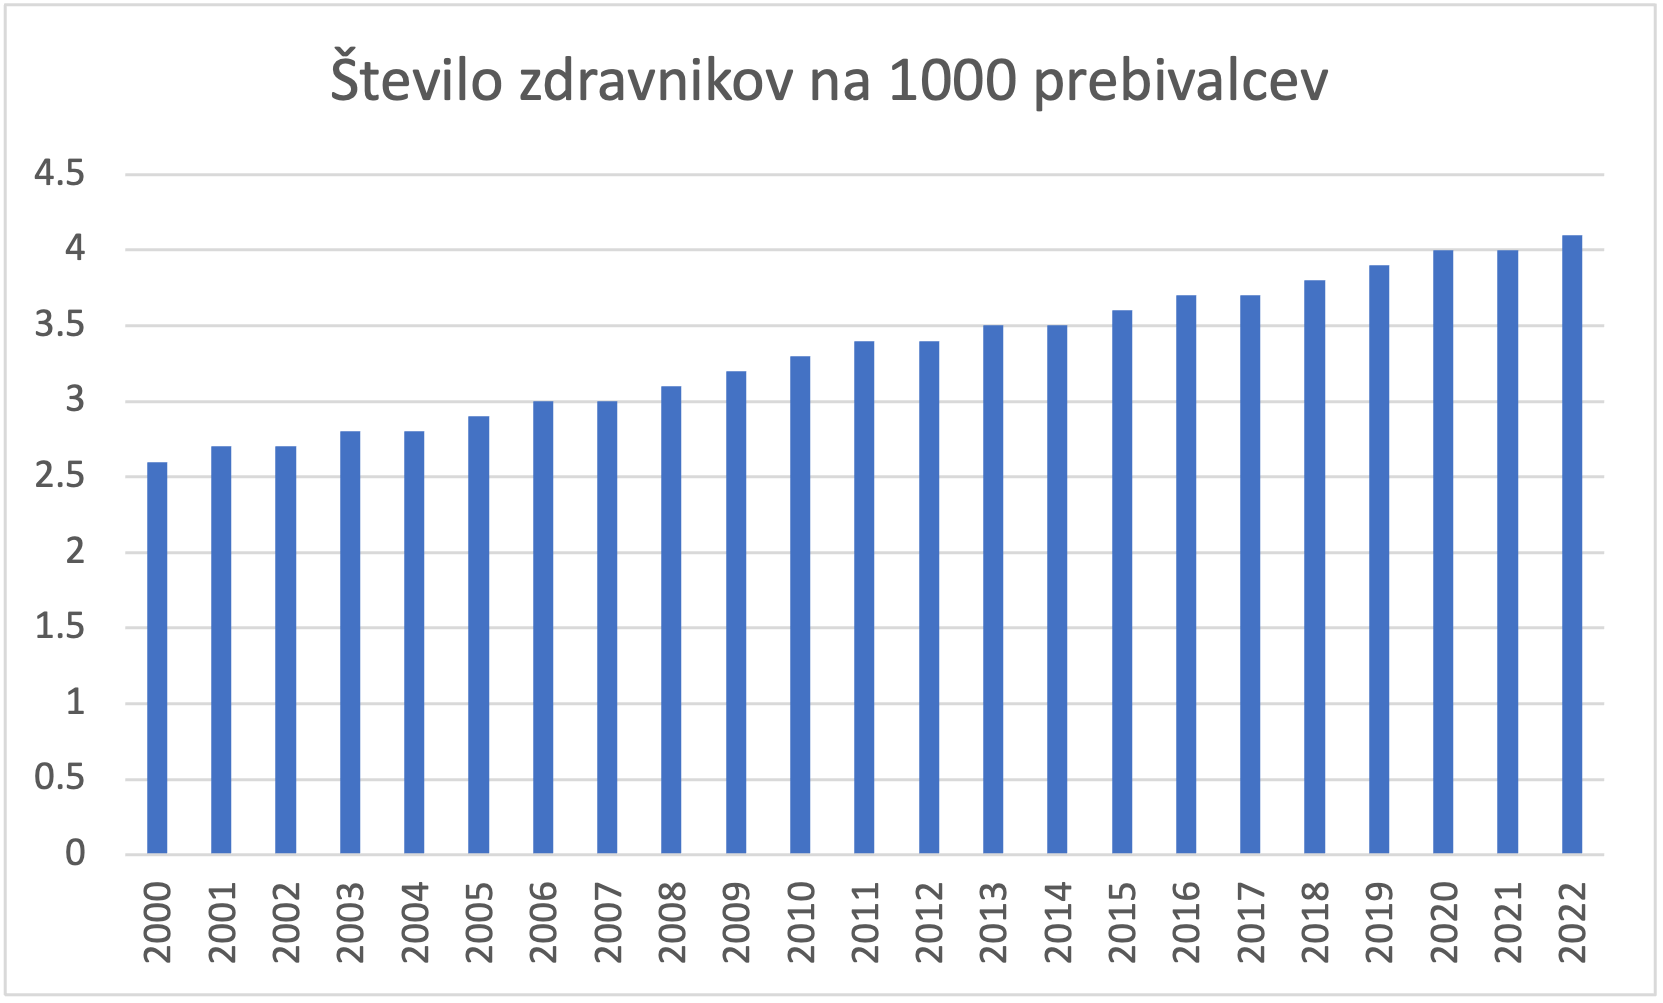
\includegraphics[width=0.7\textwidth]{zdravniki_1000_slo.png}
    \caption{Število zdravnikov v Sloveniji na 1000 prebivalcev skozi čas}
    \label{fig:zdravniki_1000_slo.png}
  \end{figure}

  \begin{figure}[H]
    \centering
    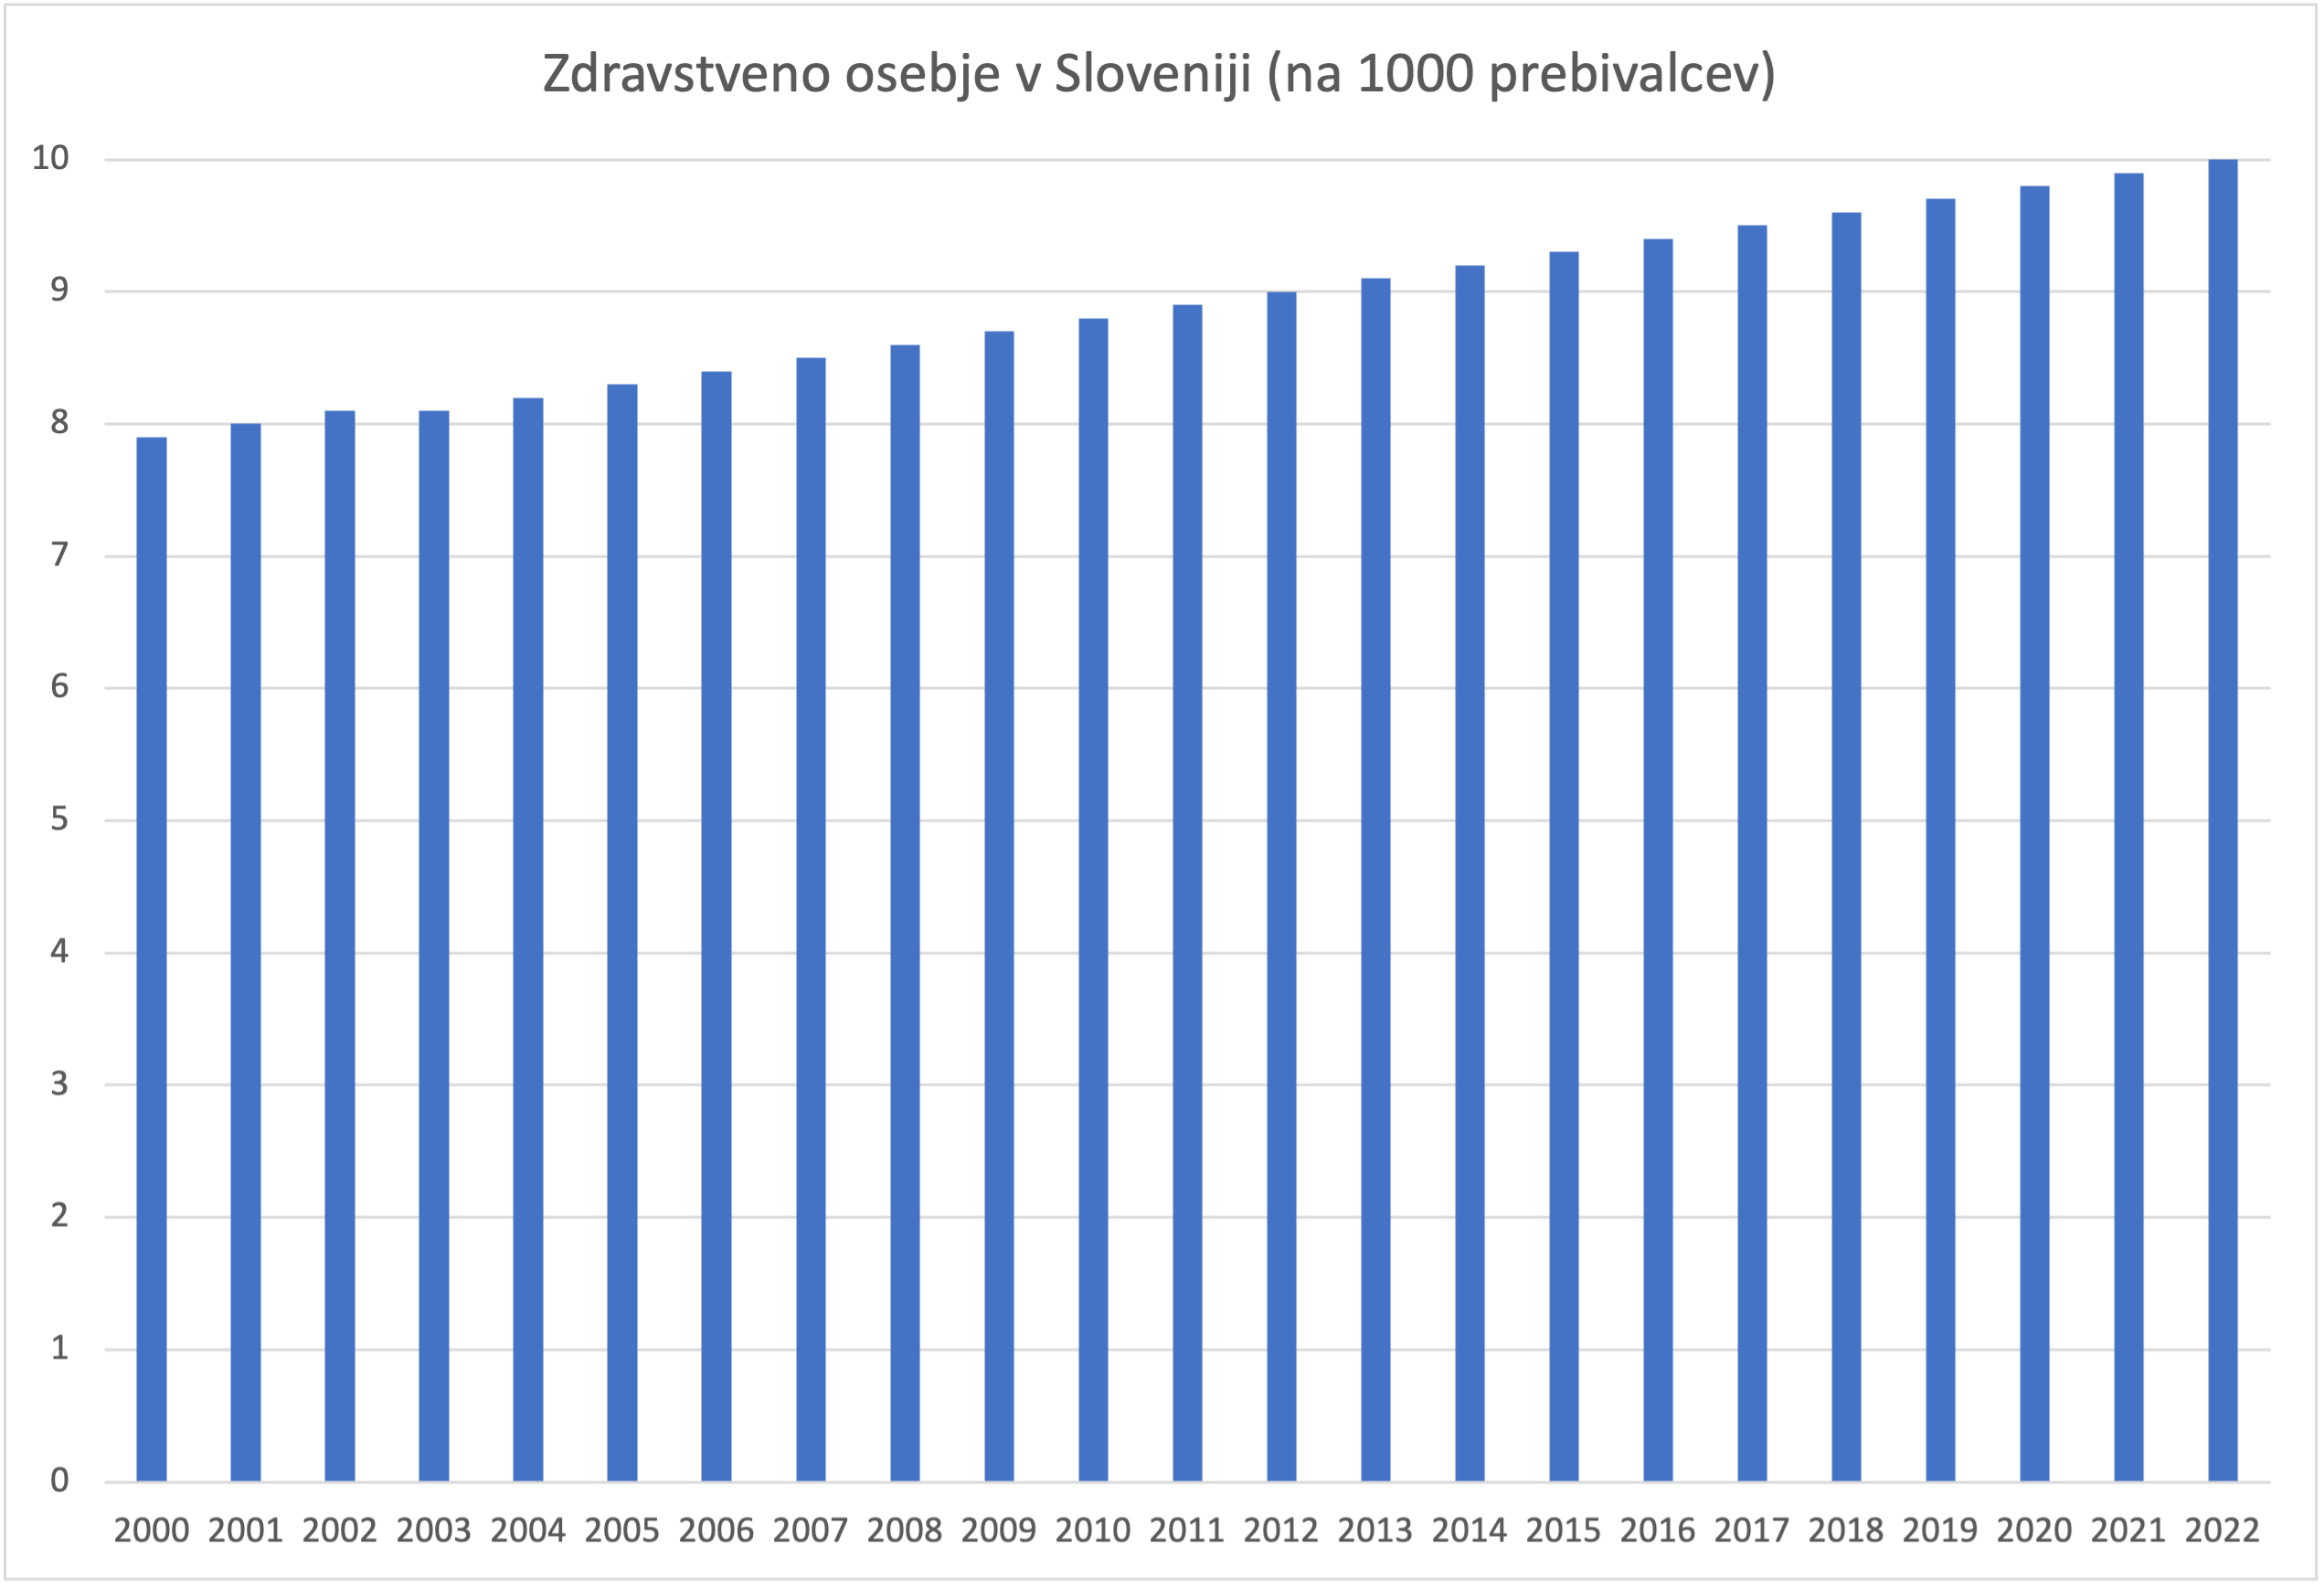
\includegraphics[width=0.7\textwidth]{zdr_osebje_1000_slo.png}
    \caption{Število zdravstvenega osebja v Sloveniji na 1000 prebivalcev skozi čas}
    \label{fig:zdr_osebje_1000_slo.png}
  \end{figure}

\subsubsection{Zdravstveni izidi}

Pri izhodih smo preučili dva kazanika, in sicer pričakovano življensko dobo državljanov in stopnjo umrljivosti dojenčkov, ki meri število umrlih otrok pred dopolnjenim prvim letom starosti na vsakih 1000 živorojenih otrok.
%zopet vir podatkov

\begin{figure}[H]
    \centering
    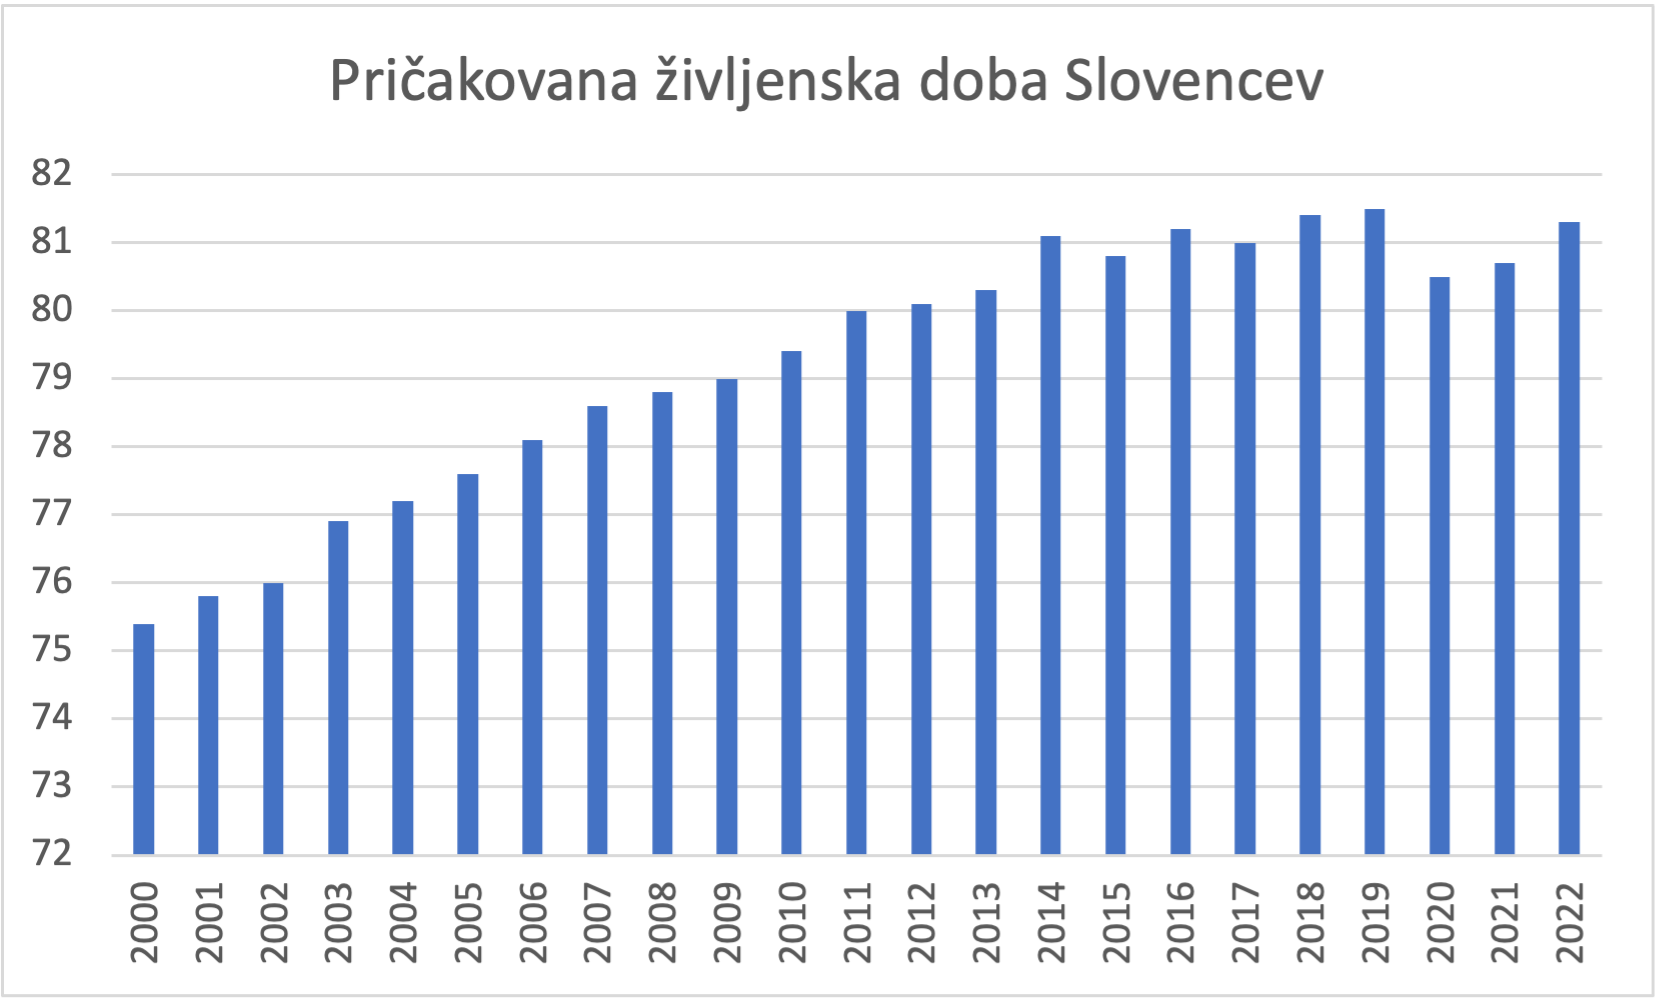
\includegraphics[width=0.7\textwidth]{pricak_zivlj_slo.png}
    \caption{Pričakovana živeljnska doba Slovencev skozi čas}
    \label{fig:pricak_zivlj_slo.png}
  \end{figure}

  \begin{figure}[H]
    \centering
    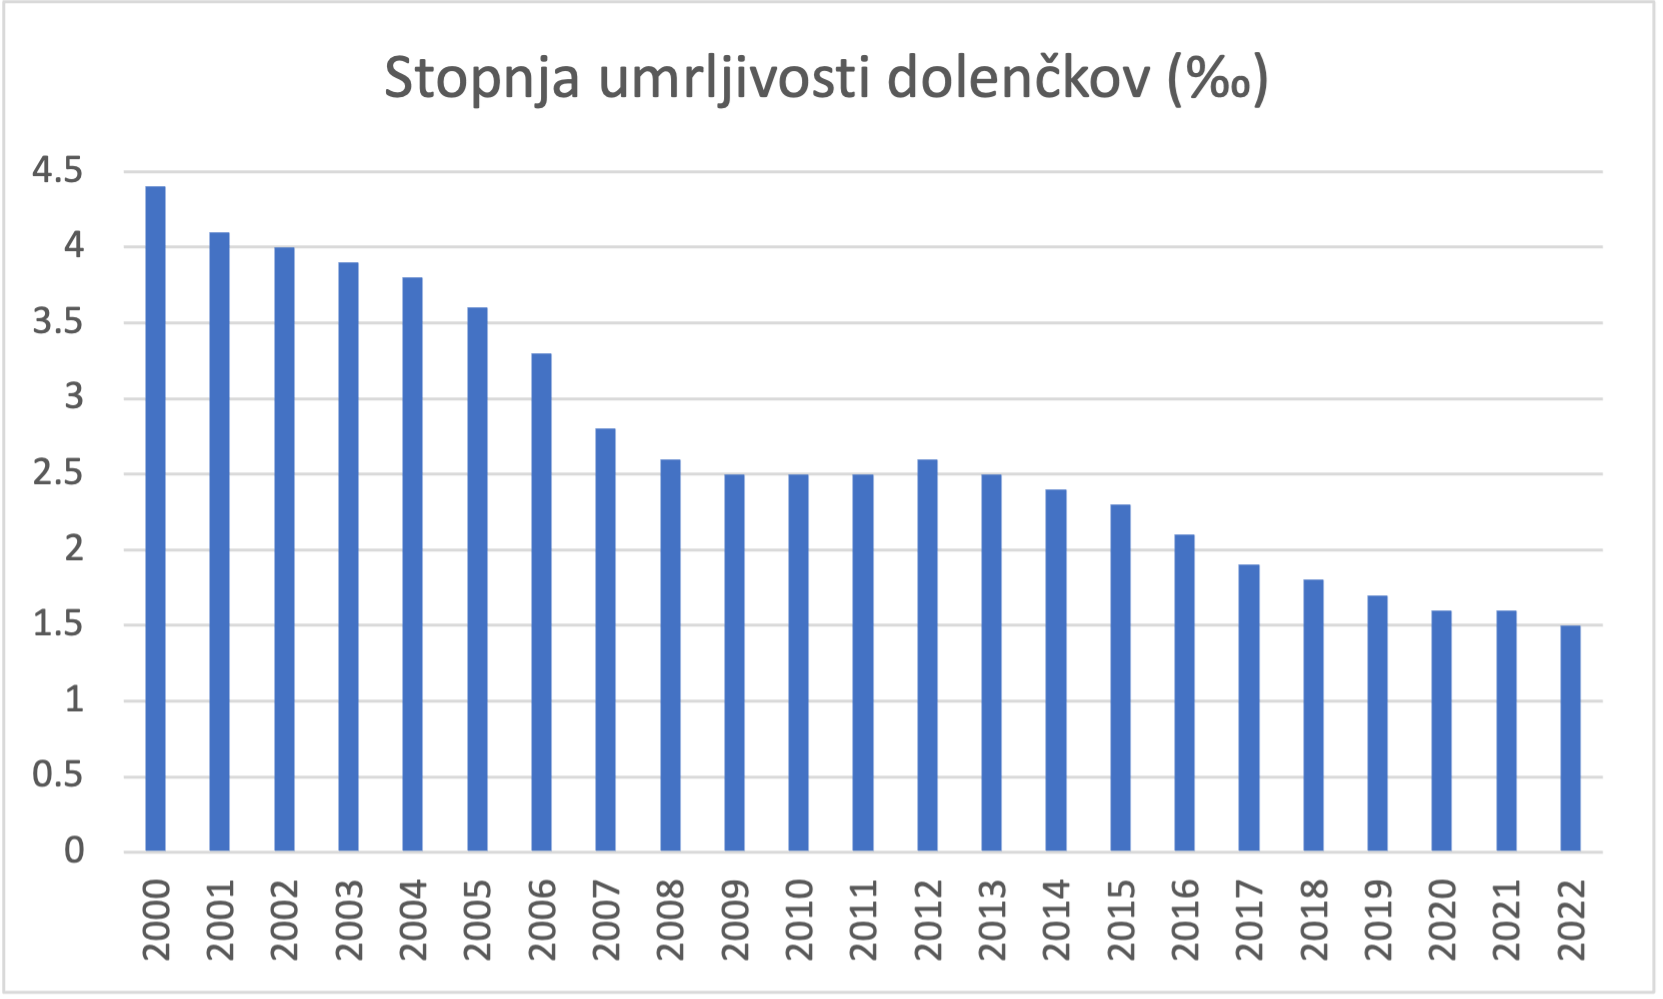
\includegraphics[width=0.7\textwidth]{umrljivost_doj_slo.png}
    \caption{Stopnja umrljivosti dojenčkov v Sloveniji skozi čas v promilih}
    \label{fig:umrljivost_doj_slo.png}
  \end{figure}

\subsubsection{CRR indeks}

  Za merjenje učinkovitosti javne porabe v zdravstvu smo uporabili Charnes-Cooper-Rhodes (CRR) model iz družine DEA metod. 
  Model primerja posamezna leta in na podlagi količine vložkov ter doseženih rezultatov ovrednoti relativno učinkovitost. 
  Vrednost 1 pomeni najvišjo relativno učinkovitost, vrednost 0 najnižjo, ostala leta pa so razvrščena vmes.

\begin{figure}[H]
    \centering
    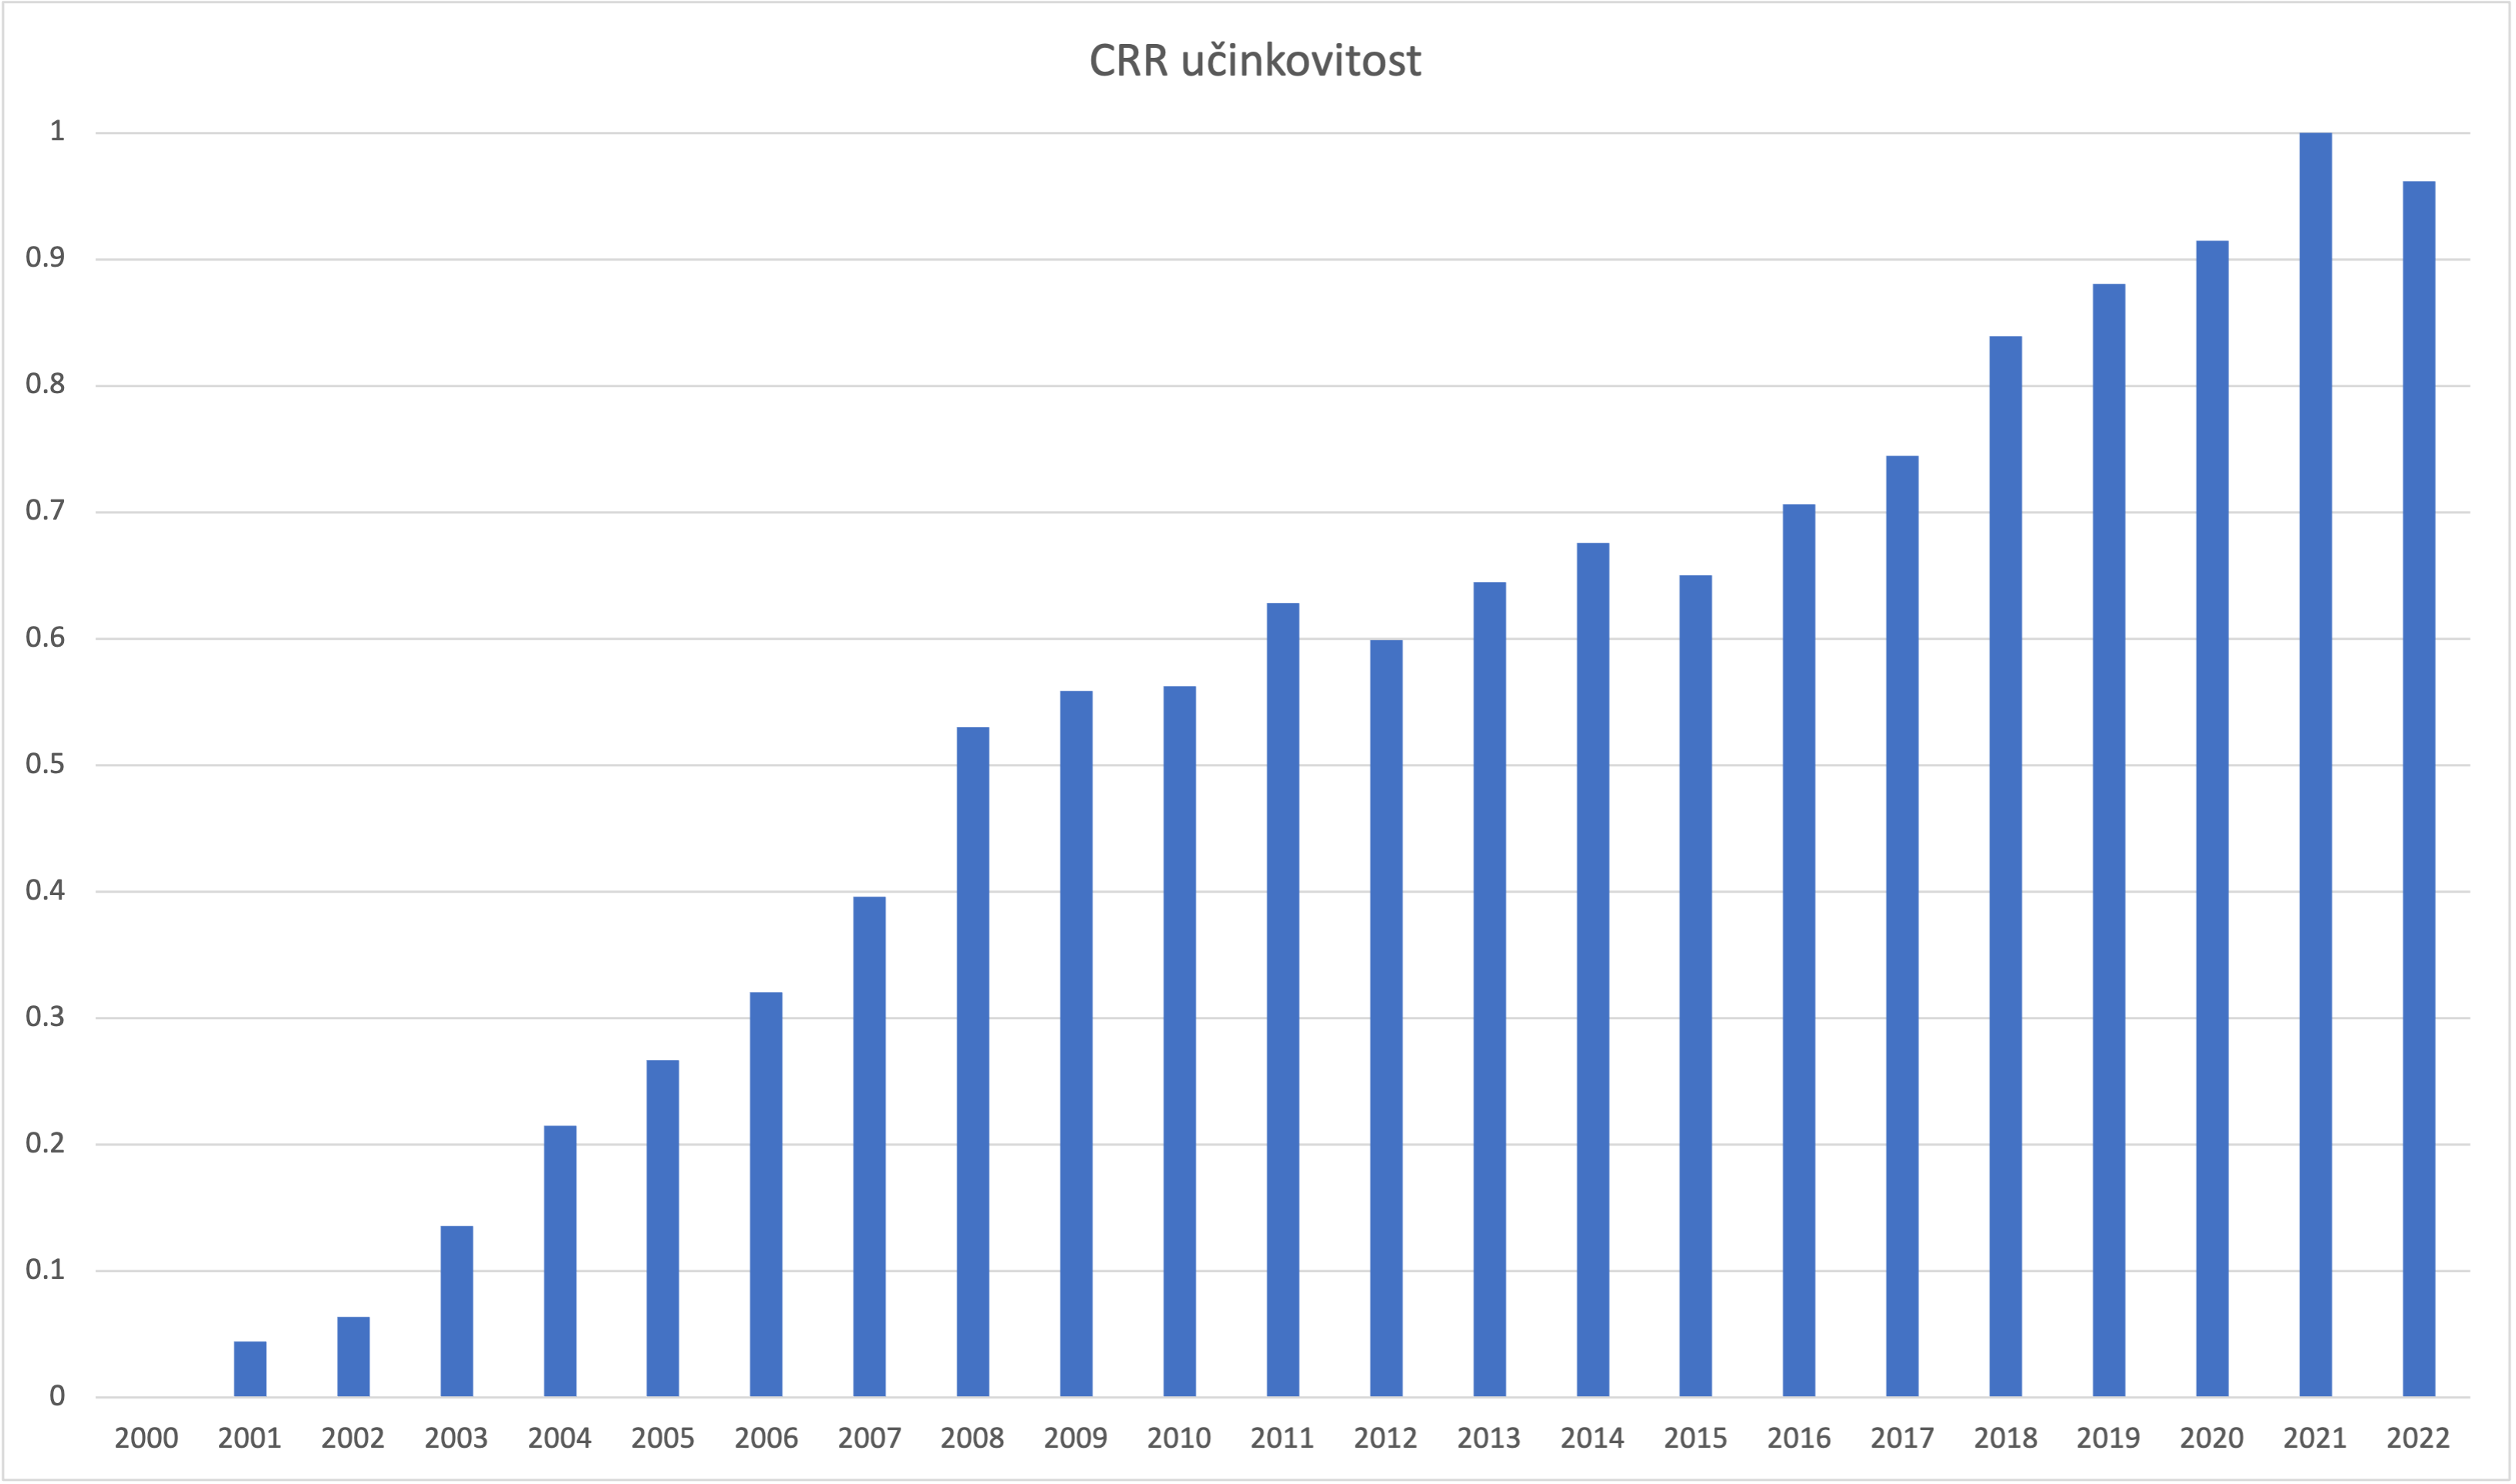
\includegraphics[width=0.7\textwidth]{CRR_stolpicni_slo.png}
    \caption{Stolpični diagram gibanja CRR indeksa slovenskega javnega zdravstva med letoma 2000 in 2022}
    \label{fig:CRR_stolpicni_slo.png}
  \end{figure}

  CRR metoda v Sloveniji pokaže zelo jasen trend v zadnjih dveh desetletjih. 
  V prvem desetletju številke konstantno rastejo, zanimivo, najmanj učinkovito leto je prav 2000. 
  Leta 2011 indeks znaša 0.628367148, naslednje leto pa prvič pade, in sicer na 0.599161023.  
  V naslednjih nekaj letih se giba nekje nad 0.6, leta 2016 pa prvič naraste nad 0.7. 
  Do izbruha epidemije COVID-19 sledi hitra rast, do najbolj učinkovitega leta, 2021, ki ima seveda indeks 1. 
  Leta 2022 učinkovitost malenkost pade, na 0.961403788.

  Učinkovitost lahko primerjamo s spremembami bruto domačega proizvoda. 
  BDP neposredno kaže obseg gospodarske aktivnosti in s tem splošno ekonomsko stanje države. 
  Za začetek velja ponoviti, da je javna poraba za zdravstvo kot delež bruto domačega proizvoda konstantno rasla, kot lahko vidimo na sliki~\ref{fig:jav_por_bdp_slo.png}. %sklic na sliko 5

\begin{figure}[H]
    \centering
    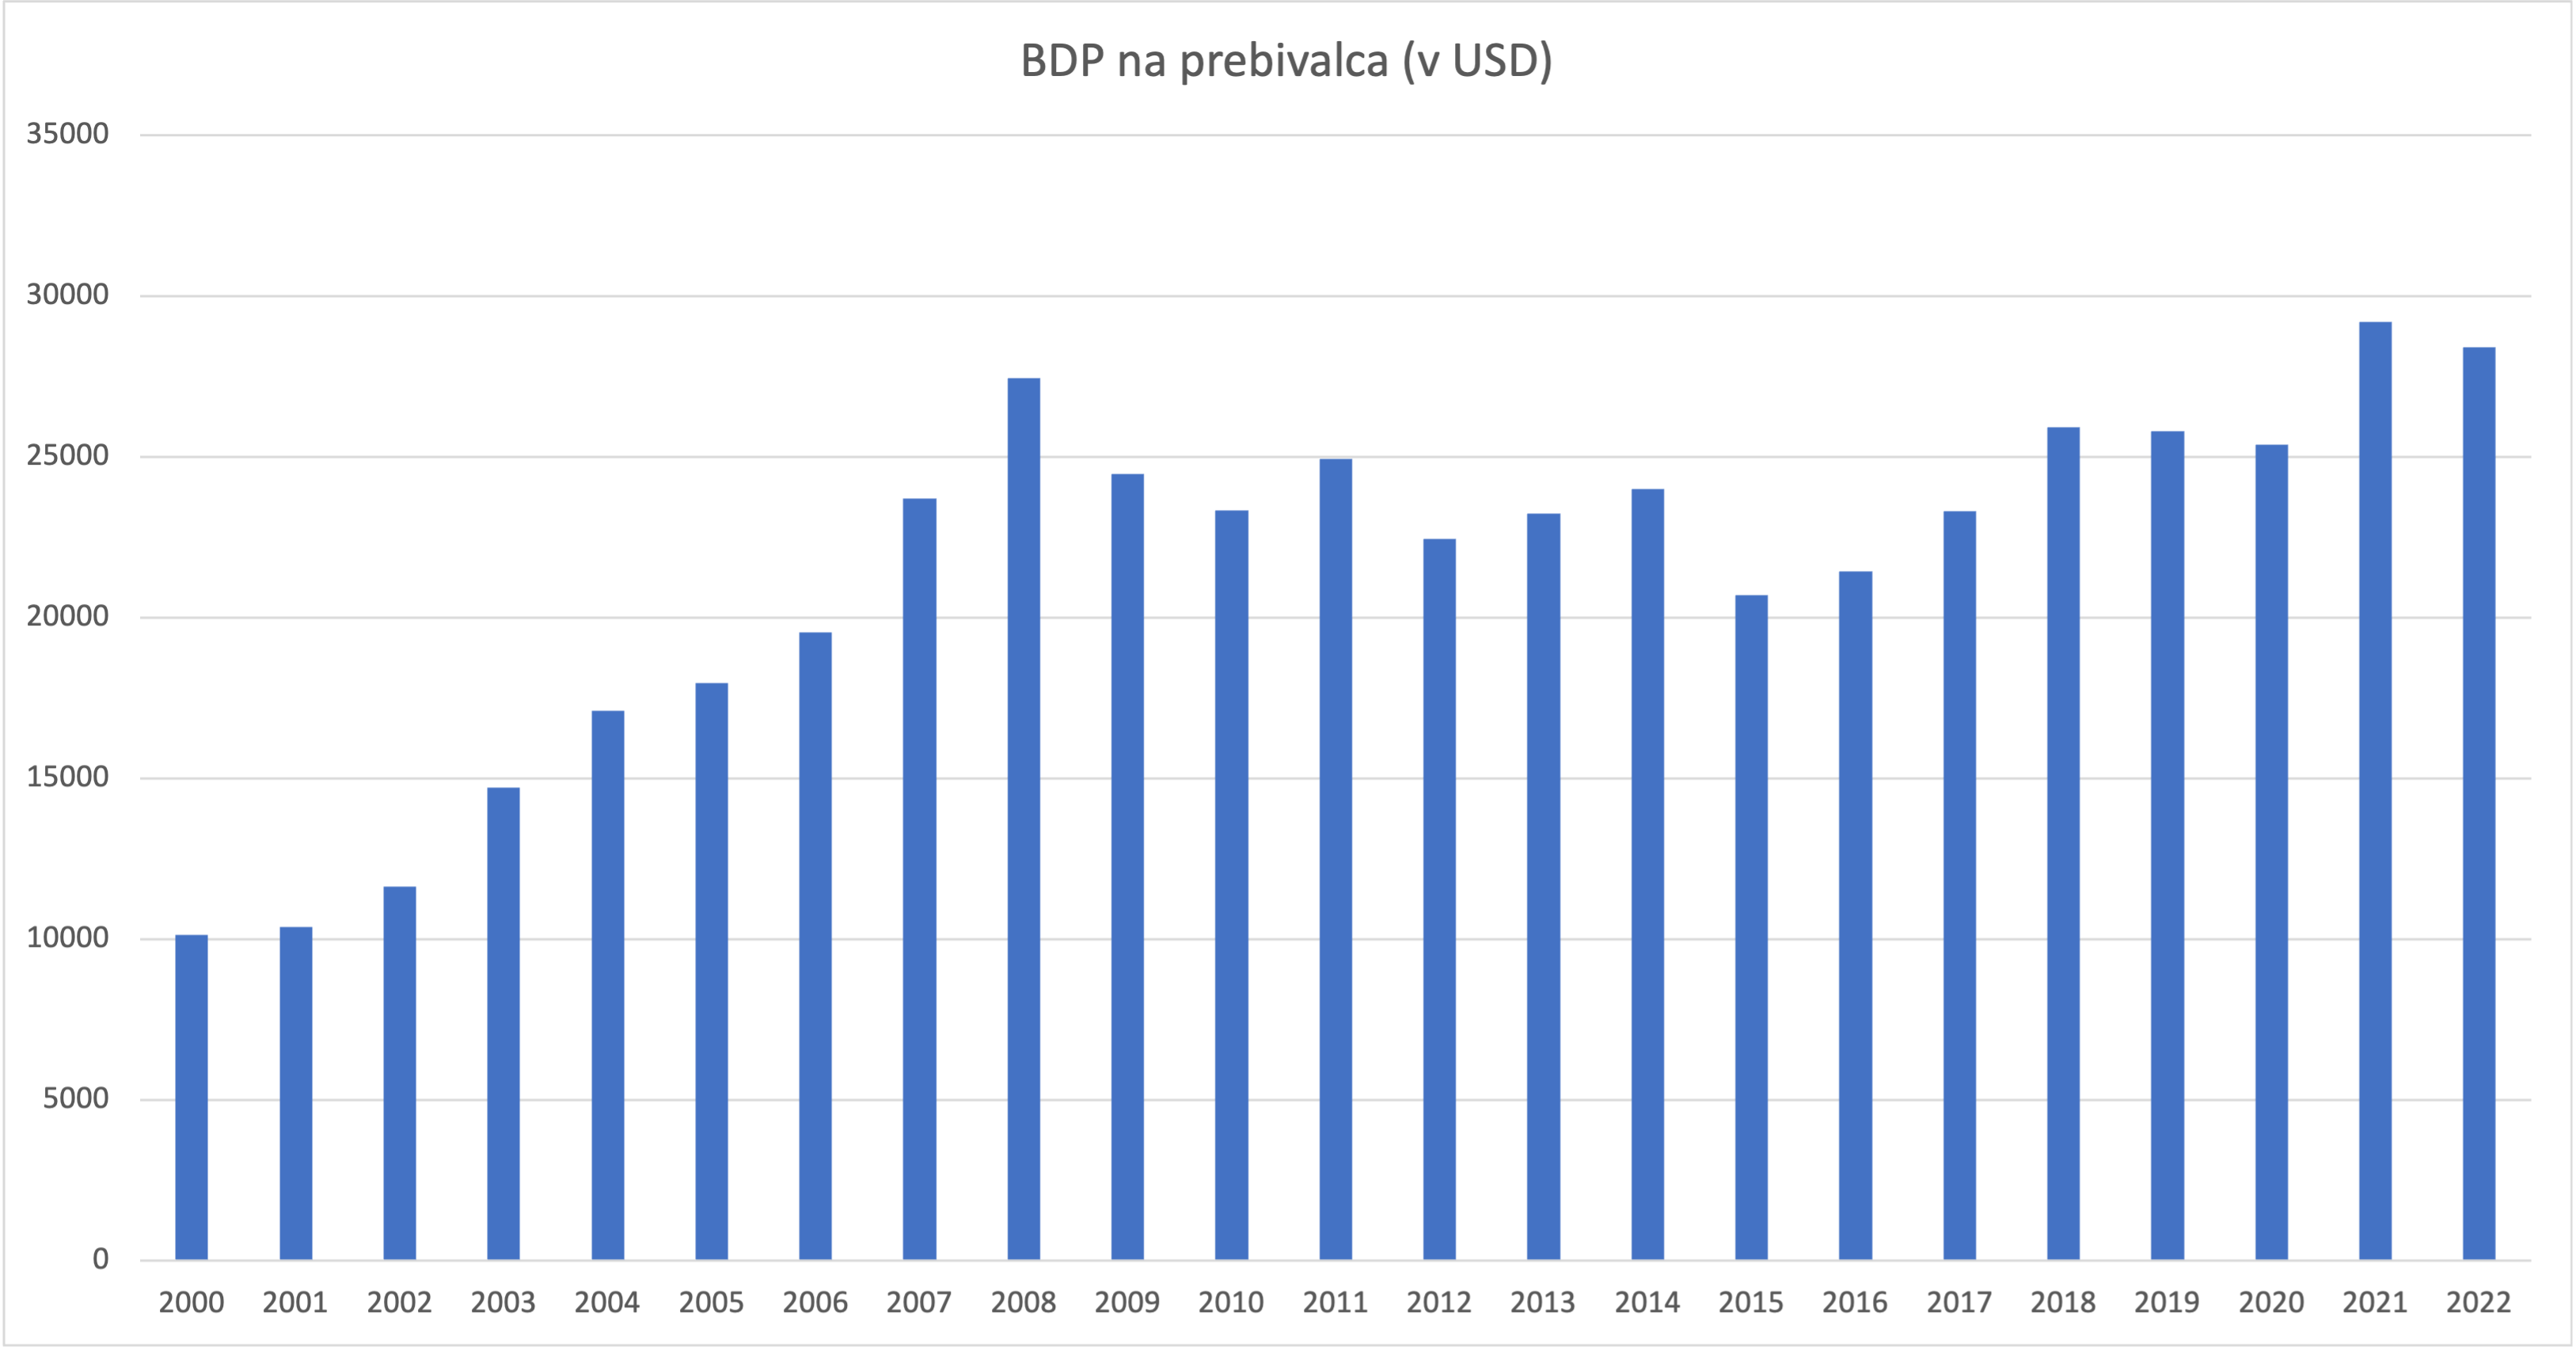
\includegraphics[width=0.7\textwidth]{bnp_pbr_slo.png}
    \caption{BDP na prebivalca v Sloveniji, v dolarjih, med letoma 2000 in 2022}
    \label{fig:bnp_pbr_slo.png}
\end{figure}

Rast BDP na prebivalca v letih do krize se ujema z večanjem učinkovitosti zdravstva, prvi padec BDP-ja v letih 2009 in 2010 pa se pri CRR indeksu še ne pozna. 
Zdi se, da je učinek gospodarske krize nekoliko zakasnjen, saj se prvi padec zgodi šele leta 2012, ko se zmanjša tudi BDP. 
V letih po krizi (od 2013 do 2018) je vzorec spremeb CRR in BDP enak, oba rasteta do 2015 in nato zopet do 2018. 

Leta 2019 je BDP na prebivalca padel za 83 evrov (kljub temu, da je celoten BDP zrastel), padec je sledil tudi leta 2020 (na prebivalca in celostno). 
Učinkovitost tu ne sledi trendu gospodarstva, saj do leta 2021 raste do svojega »najboljšega rezultata«. 
Leta 2021 se je gospodarstvo po pandemiji pobralo, kar se odraža tudi v večjem skoku BDP na prebivalca. 
Najbolj učinkovito leto v zdravstvu je tako tudi leto z najvišjo gospodarsko aktivnostjo v preučevanem obdobju.

Ob tem je zanimivo, da je Komisija za preprečevanje korupcije v svoji analizi delovanja javnega sektorja na področju zdravstva opozorila, da je epidemija povečala sistemske izzive. 
Ob kriznem delovanju so se povečala tveganja povezana s korupcijo, opazili so netransparentnost pri naročilih in pogrešali več objavljenih podatkov o izvedenih naročilih. 
\cite{analizaJavnegaZdravstva2023} 

Analiza ministrstva za zdravje je pokazala, da je bila dostopnost zdravstvenih storitev v letih 2020 in 2021 na splošno zmanjšana in okrnjena. 
Za okoli 20 odstotkov so upadle obravave v ambulantah in hišne obravnave. Zelo okrnjeni so bili tudi preventivni programi (Zora, Dora in Svit), število preventivnih pregledov odraslih se je zmanjšalo za več kot pol. 
Zabeleženo je bilo le 70 odstotokv realiziranih napotnic glede na število izdanih, kar pomeni, da velik del pacientov ni prišel do načrtovanih pregledov. \cite{jamsek2022analiza}

CRR indeks kljub omenjenim težavam kaže, da je v izrednih razmerah zdravstvo delovalo najboljše. Pri ugotovitvah je potrebno upoštavati, da števila opravljenih pregledov v analizo nismo vključili, tako da je učinkovitost med epidemijo treba vzeti z rezervo.

Vseeno velja omeniti, da je COVID-19 imel tudi pozitivne učinke na učinkovitost, poročila predvsem izpostavljajo digitalizacijo.


\subsubsection{Malmquistov indeks}
Malmquistov indeks meri spremembo skupne produktivnosti med dvema zaporednima letoma. 
Vrednost nad 1 pomeni napredek, vrednost 1 stabilnost, medtem ko vrednost pod 1 kaže na upad produktivnosti. 
Indeks zajema vpliv tehnološkega napredka in učinkovitostnih prilagoditev. Primarno se ga uporablja za analizo v podjetjih, 
zato pri preučevanju javnega sektorja ne vidimo nekih pretiranih odstopanj. 
Tako je bilo tudi v Sloveniji, kjer so spremebe glede na prejšne leto ostale znotraj 0,985 in 1,015.

\begin{figure}[H]
    \centering
    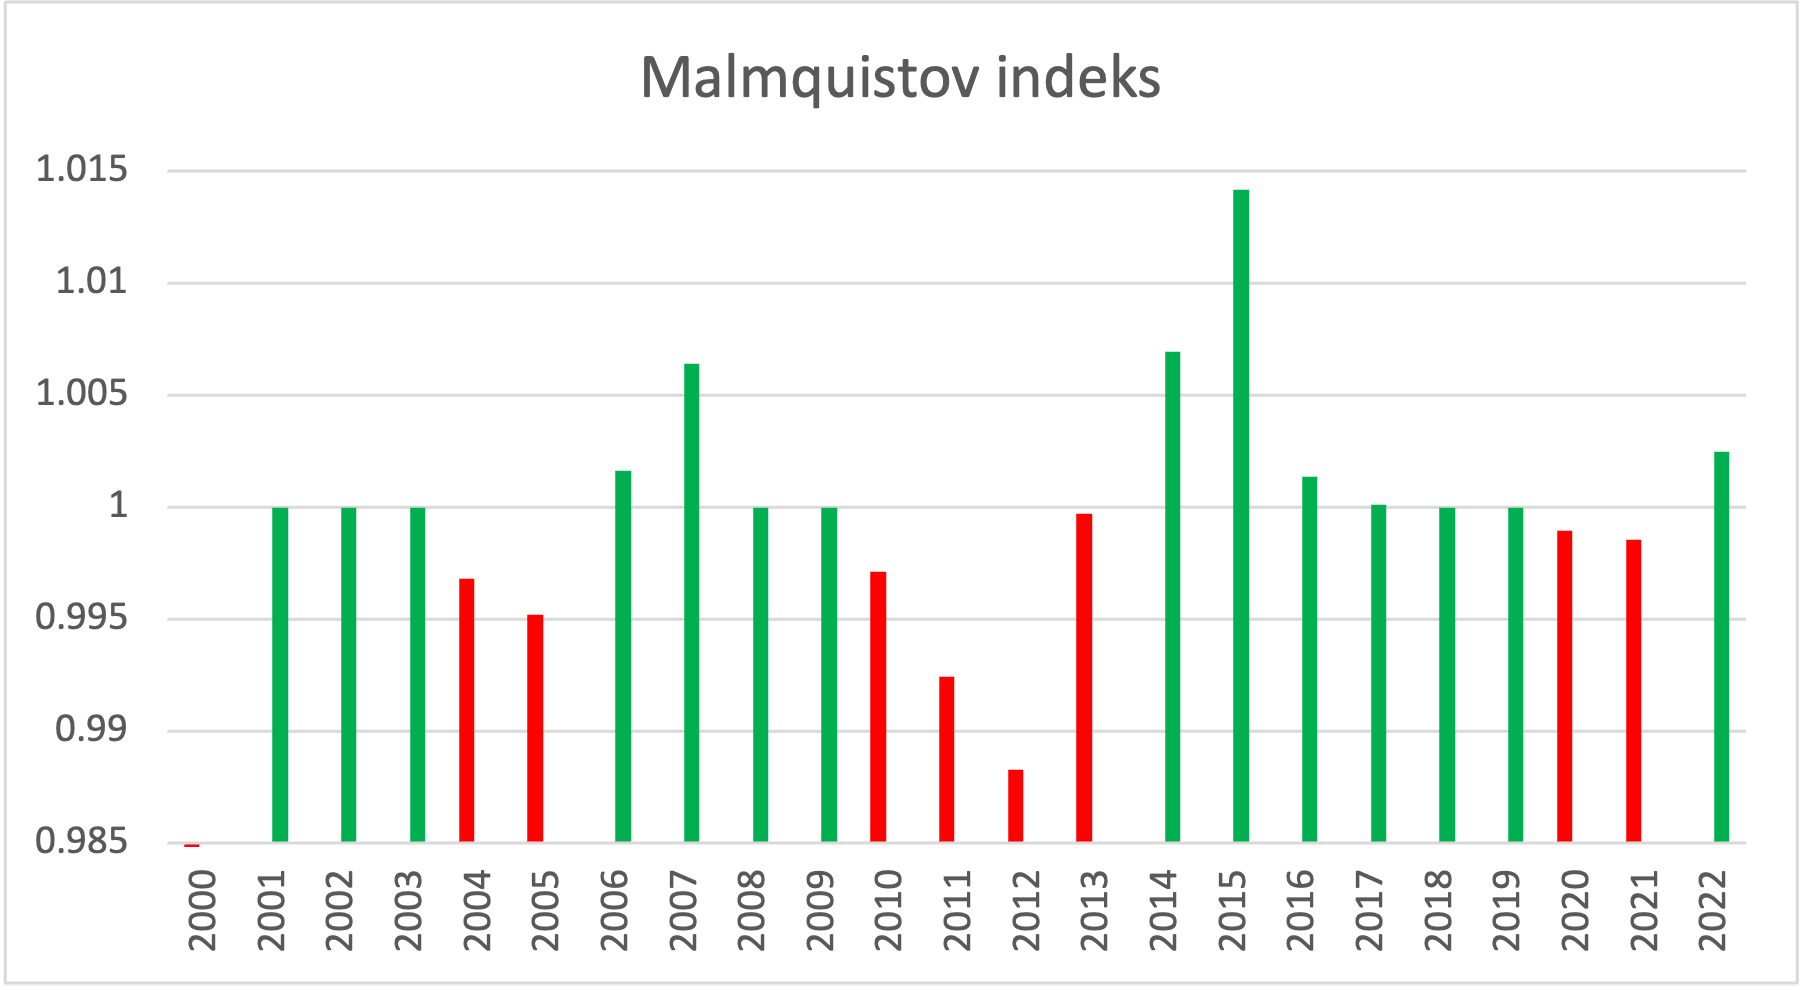
\includegraphics[width=0.7\textwidth]{malmq_ind_slo.png}
    \caption{Malmquistov indeks učinkovitosti javnega zdravstva v Sloveniji med letoma 2000 in 2022}
    \label{fig:malmq_ind_slo.png}
\end{figure}

\section{Zaključek}

Analizirali smo učinkovitost javenga zdravstva v Sloveniji in ZDA
v obdobju 2000--2022. S pomočjo CRR indeksa in zbranih podatkov
smo prišli do zaključka, da je učinkovitost tako v Sloveniji kot
v ZDA naraščala in dosegla višek v letu 2020 v času COVID-19. To smo
razložili prek postopnega dvigovanja deleža izdatkov BPD-ja za zdravstvo in
dviga števila zdravstevnih delavcev.

Malmquistov indeks nam je pokazal, da sta produktivnosti v Sloveniji
in ZDA relativno stabilni, pomembno pa je vseeno omeniti velik padec
učinkovitosti v letu 2022 v ZDA. Izziv za obe državi v prihodnje bo ohranjanje izboljšav in nadaljna optimizacija,
še posebej ob upoštevanju staranja prebivalstva.

\nocite*{}
\bibliographystyle{apalike}
\bibliography{javni_sektor}

\end{document}
